%% Choose language: english or german
%% Choose Thesis type: seminar, bachelor, master, techreport
\documentclass[english,techreport]{IPRthesis}

%% ---------------------------------
%% | Information about the thesis  |
%% ---------------------------------
% TODO: Change this \titleenglish \titlegerman. Same for keywords.
\title{Implementierung eines Clusteringbasierten Verfahrens zur Visualisierung von Volumenmodellen}
\titleotherlanguage{Mein Titel\\
ist lang}

\author{Lukas Diewald}

\keywords{Keywords, of, my, Thesis}
\keywordsotherlanguge{Die, Stichw\"orter, f\"ur, meine, Arbeit}

%% Study program or for seminars name of a seminar
\studyprogram{Intelligente Industrieroboter}

\reviewerone{Prof. Dr.-Ing. habil. Björn Hein}
\reviewertwo{Prof. B}
%
% %% The advisors are PhDs or Postdocs
\advisorone{M.Sc. C}
% %% The second advisor can be omitted
\advisortwo{M.Sc. D}
%
% %% Please enter the start end end time of your thesis
\editingtime{xx. Month 2018}{xx. Month 2018}

%% --------------------------------
%% | Settings for word separation |
%% --------------------------------
% Help for separation:
% In german package the following hints are additionally available:
% "- = Additional separation
% "| = Suppress ligation and possible separation (e.g. Schaf"|fell)
% "~ = Hyphenation without separation (e.g. bergauf und "~ab)
% "= = Hyphenation with separation before and after
% "" = Separation without a hyphenation (e.g. und/""oder)

% Describe separation hints here:
\hyphenation{
% Pro-to-koll-in-stan-zen
% Ma-na-ge-ment  Netz-werk-ele-men-ten
% Netz-werk Netz-werk-re-ser-vie-rung
% Netz-werk-adap-ter Fein-ju-stier-ung
% Da-ten-strom-spe-zi-fi-ka-tion Pa-ket-rumpf
% Kon-troll-in-stanz
}


%% ------------------------
%% |    Including files   |
%% ------------------------
% Only files listed here will be included!
% Userful command for partially translating the document (for bug-fixing e.g.)
% \includeonly{%
% Content/0-Declaration,
% Content/0-Abstract_EN,
% Content/0-Abstract_DE,
% Content/1-Introduction,
% Content/2-State-of-the-art,
% Content/3-Methods,
% Content/4-Concept,
% Content/5-Implementation,
% Content/6-Results,
% Content/7-Discussion,
% Content/8-Conclusion,
% Content/11-Appendix,
% }

\settitle
%%%%%%%%%%%%%%%%%%%%%%%%%%%%%%%%%
%% Here, main documents begins %%
%%%%%%%%%%%%%%%%%%%%%%%%%%%%%%%%%
\begin{document}

%% Set PDF metadata
\setpdf

%% Set the title
\maketitle

% TODO: Remove this from final version
\newpage
\listoftodos
\newpage

\includedeclaration

\includeacknowledgments

\setcounter{page}{1}
\pagenumbering{roman}

%% ----------------
%% |   Abstract   |
%% ----------------
%% An abstract both in English
%% and German is mandatory.
%%
%% The text is included from the following files:
%% - Content/0-Abstract_EN
%% - Content/0-Abstract_DE
\includeabstract

%% ------------------------
%% |   Table of Contents  |
%% ------------------------
\inculdetableofcontents

\makenomenclature

%% -----------------
%% |   Main part   |
%% -----------------

\setcounter{page}{1}
\pagenumbering{arabic}
%% ==============================
\chapter{\iflanguage{ngerman}{Einleitung}{Introduction}}
\label{sec:Introduction}
%% ==============================

As an useful aid in all scientific work following book is recommended: \cite{deininger1992studienarbeiten}

\todo{Rewrite this seciton}
\nomenclature{IAR-IPR}{Institute for Anthropomatics and Robotics (IAR) - Intelligent Process Control and Robotics (IPR)}

%% ==============================
\chapter{\iflanguage{ngerman}{Stand der Wissenschenschaft und Technik}{State of the art}}
\label{sec:state_of_the_art}
%% ==============================




%%Bajaj Countour: \cite{bajaj1997contour} -1d


Das Gebiet der Transferfunktionen ist bereits weit erforscht und es existieren viele unterschiedliche Methoden und Herangehensweisen um medizinische Daten abhängig von verschiedenen Problemstellungen passend darzustellen.
\newline
Dabei ist zwischen dem Level an Automation eines Systems zu unterscheiden. Hierbei gibt es vollautomatische Verfahren, bei denen keine Interaktion mit dem Benutzer von Nöten ist, semiautomatische Verfahren bei denen der Benutzer noch an gewissen Stellschrauben drehen kann um das Ergebnis zu beeinflussen und manuelle Verfahren, bei denen der Anwender vieles selbst einstellen muss. Transferfunktionen unterscheiden sich weiterhin in ihrer Dimensionalität. Es existieren ein- zwei- und allgemein -mehrdimensionale Transferfunktionen.
Des Weiteren sind die Grundlagen auf denen die Berechnungen ruhen teils völlig verschieden. Manche Verfahren basieren auf den Intensitätswerten oder deren Änderung im gegebenen Volumen. Andere basieren auf der Größe der Features die für den Nutzer von Interesse sind. Wieder andere sind Benutzer-zentrisch orientiert oder wenden Machine Learning an um zu einem gewünschten Ergebnis zu gelangen.
\newline
In diesem Abschnitt wird ein Überblick über die unterschiedlichen Vorgehensweisen von Transferfunktionen gegeben. Dazu werden diese im Folgenden in die Unterkapitel Eindimensionale, Zweidimensionale, Raum-basierte, Machine Learning, Benutzer-zentrische und Clustering-basierte Verfahren aufgeteilt.
Eine Einteilung in verschieden Kategorien fällt dabei schwer, da viele der Verfahren mehrere der genannten Herangehensweisen verbinden. Aus diesem Grund können manche Verfahren nicht eindeutig in die hier genannte Unterteilung eingeteilt werden, da eine Mehrfachnennung möglich wäre.


\subsection{Eindimensionale Verfahren}

Die einfachste Form einer Transferfunktionen, ist eine eindimensionale. Bei dieser wird einem Voxel Farbe und Okklusion nur abhängig von dessen Intensitätswerten zugeteilt.
\newline
Abgesehen von den niedrigen Berechnungszeiten, eigenen sich diese aus mehreren Gründen nicht, um das Ventrikelsystem zu segmentieren. Medizinischen Daten werden gemessen und haben deshalb meist ein Rauschen, was die genaue Darstellung erschwert. Weiterhin sind die Intensitätswerte verschiedener Bereiche nah beieinander oder gar gleich. Deshalb sind eindimensionale Transferfunktionen unpraktisch um verschiedene Materialien kenntlich zu machen.
\newline
Trotzdem sind eindimensionale Transferfunktionen weit verbreitet und werden häufig benutzt, da sie oft bei Softwarepaketen inklusive sind.


Eine etwas komplexere eindimensionalen Transferfunktion wird im Paper von Drebin \cite{drebin1988volume} vorgestellt, bei der Voxel, anhand von Wahrscheinlichkeiten, die auf den Intensitätswerten basieren, klassifiziert werden. Abhängig von dieser Klassifizierung werden den Voxeln Farbwerte zugewiesen.



\subsection{Zweidimensionale Verfahren}

Bei zweidimensionalen Transferfunktionen werden häufig als zweite Eingabegröße neben den Intensitätswerten die Länge der Gradienten hinzugezogen. Der Gradient eines Voxels, ist ein Vektor, der in die Richtung der größten Änderung der Intensitätswerte zeigt.


Ein frühes Beispiel für die Verwendung der Gradientenlänge, ist aus dem Jahr 1988 aus dem Paper von Levoy \cite{levoy1988display}. In diesem werden, mithilfe einer simplen Funktion, Voxeln Opazitätswerte abhängig von deren Intensitätswerten und Gradientenlängen zugewiesen.


Kniss stellt in seiner Arbeit \cite{kniss2002multidimensional} ebenfalls Transferfunktionen vor, die auf Intensitätswerten und Gradientenlängen basieren. Der Benutzer kann über eine graphische Oberfläche sogenannte \textit{widgets} auf dem zweidimensionalen Histogramm erstellen, welche die Visualisierung der Daten bestimmen.


Das Paper von Shouren Lan \cite{lan2017improving} befasst sich hingegen mit der Verbesserung solcher zweidimensionalen Transferfunktionen die auf Skalarwerten und Gradienten(kurz: SG-TF) basieren.
Genauer geht es darum, die bei solchen Transferfunktionen immer wieder vorkommende Überlappung von unterschiedlichen Bereichen zu verbessern.
Dabei wird im Paper zwischen 3 verschiedenen Klassen von Strukturen unterschieden:
\begin{itemize}
\item (i) Strukturen die keine andere Struktur berühren
\item (ii) Strukturen die keine andere Struktur berühren, jedoch nah an einer anderen liegen
\item (iii) Strukturen die andere Strukturen berühren
\end{itemize} 
Wenn der Benutzer eine Region ausgewählt hat, werden zunächst alle Strukturen in dem Bereich klassifiziert und kleine Fragmente entfernt. Durch verschiedene Algorithmen werden Strukturen der Klassen (ii) durch Erosion, Dilatation, Aufteilen und neu zusammenfügen von einander getrennt. Strukturen der Klasse (iii) werden durch eine weitere niedrig dimensionale Transferfunktion getrennt.
Anschließend werden Löcher, die beim Aufteilen der Strukturen entstehen mithilfe von einem Dilatationsoperator geschlossen. Als letztes wird den unterschiedlichen Strukturen verschiedene Farben und Okklusionen zugewiesen.
\newline
Das Vorgehen von Lan führt zwar zu guten Ergebnissen und wurde sogar schon am Ventrikelsystem getestet, jedoch wäre die Implementierung des Verfahrens mit der Unterscheidung der Klassen und den verschiedenen Algorithmen zum Teilen der Strukturen, Schließen von Löchern etc. sehr zeitaufwändig und damit im Rahmen dieser Bachelorarbeit  nicht umsetzbar.



\subsection{Raum-basierte Verfahren}

In der Arbeit von Wesarg und Kirschner \cite{wesarg2009structure, wesarg20102d} wird das \textit{Stucture-Size-Enhanced Histogram} vorgestellt.
Zur Berechnung des Histogramms  muss für jeden Voxel die Strukturgröße abgeschätzt werden. Dies geschieht, indem die Anzahl an Schritten, die in die jeweiligen Richtungen der 26 Nachbarvoxel vollbracht werden kann, aufaddiert wird. Ein Schritt kann ausgeführt werden, wenn der Intensitätswert des erreichten Voxels nicht mehr als ein gegebener Parameter von dem Intensitätswert des Ausgangspunkt abweicht.
\newline
Der erste Schritt hat eine Länge von einem Voxel, der zweite von zwei Voxeln, der dritte von vier Voxeln... und so weiter. Die Schrittweite verdoppelt sich mit jedem weiteren Schritt bis hin zur Hälfte der Größe des gesamten Volumens. Hierbei kann ein Schritt trotzdem nur ausgeführt werden, wenn alle Voxel auf dem Weg das Kriterium erfüllen. Die Akkumulation alle Werte ergibt die geschätzte Größe der Struktur des Voxels. Dabei wird, um das Ergebnis weiterhin zu verbessern,  jeweils nur der kleinere Wert von zwei entgegengesetzten Richtungen in der Berechnung verwendet. 
Aus der geschätzten Größe und dem Intensitätswert wird ein zweidimensionales Histogramm erstellt. Abhängig von der euklidischen Distanz der Kästchen des Histogramms zu einem vom Benutzer gegebenen Punkt, werden die Farbwerte der einzelnen Voxel aus einer Farbtabelle ausgelesen.
\newline
Das Verfahren eignet sich gut, um relativ große Strukturen zu erkennen, jedoch ist es unklar ob das relativ schmale Ventrikelsystem erkannt werden würde.


Eine andere Idee Strukturen basierend auf räumlichen Informationen zu Segmentieren ist die Verwendung von Region Growing.
Beispielsweise wird im Paper von Huang \cite{huang2003rgvis} ein solches Regiongrowingverfahren vorgestellt. Der Benutzer kann einen Punkt von Interesse im Volumen wählen, den sogenannten \textit{seed}. Es werden alle 26 Nachbarn des \textit{seeds} besucht und anhand einer Kostenfunktion, die den entsprechenden Wert des besuchten Voxels und des \textit{seed}-Voxels vergleicht, entschieden ob sie zu der Region dazugehören oder nicht. Sind sie Teil der Struktur werden auch ihre Nachbarn besucht und alle passenden Voxel zu der Region hinzugefügt. Diese Vorgang wiederholt sich so lange bis alle Voxel gefunden wurden, oder ein anderes internes Abbruchkriterium erfüllt wurde.
\newline
Es stehen dem Anwender drei verschiedene Kostenfunktionen zu Verfügung. Die erste Funktion bezieht sich auf die Intensitätswerte der Voxel, die Zweite auf die Länge der jeweiligen Gradienten und bei der Dritten werden die Gewichte der Voxel verglichen, die vorher vom Benutzer definiert werden müssen.
In einem Nachbearbeitungsschritt ist es anschließend noch möglich Elemente, die nicht zur Struktur von Interesse gehört, zu entfernen, wenn beispielsweise eine ganze weitere Struktur auch visualisiert wird, da sie über eine kleine Brücke von ein bis zwei Voxeln mit der eigentlich gesuchten Struktur verbunden ist.
Da das Regiongrowing sehr zeitaufwändig ist, kann der Anwender auswählen, dass er zunächst nur eine gewisse Teil der Region sich errechnen lässt.


Im Vergleich zu Huan \cite{huang2003rgvis} benutzt Chen  in seiner Arbeit \cite{chen2006sketch} nicht nur ein \textit{seed}basiertes Vorgehen, sondern fügt noch ein sketchbasiertes Verfahren davor ein.
Anfangs wählt der Anwender eine Reihe an Intensitätswerten im Histogramm, die für ihn interessant sind. Danach kann er direkt im Volumen eine Region von Interesse einzeichnen und markieren. Das Programm schneidet im Anschluss, alle Teile des Volumens, die außerhalb der gewählten Region liegen, weg. Jetzt kann der Nutzer wie im vorherig vorgestellten Verfahren seinen \textit{seed} setzen.
Dies erleichtert dem Benutzer die Anwendung, da er schneller zu seinem Punkt von Interesse gelangt ohne vorher durch diverse Querschnittbilder iterieren zu müssen. Des Weiteren ist es zeitsparend für den User, falls dieser sich nicht genau mit dem Datensatz und der zu Visualisierenden Region auskennt.


Correa und Ma zeigen in ihrer Arbeit \cite{correa2008size} hingegen einen Ansatz, der auf der relativen Größe der zu visualisierenden Features basiert.
Dazu benutzen sie den sogenannten \textit{scale-space}, welcher für das Volumen berechnet wird, um anschließend eine auf Größe basierende Transferfunktion anzuwenden. Diese ordnet Farbe und Okklusion den entsprechenden Größen der Features des Volumens zu.


In einem weiteren Paper \cite{correa2009occlusion} beschreiben die beiden Forscher ein Verfahren, dass auf der Okklusion der Voxel basiert.
Dafür betrachten sie die Umgebung einzelner Voxel und berechnen abhängig davon, die Okklusion. Die Ergebnisse werden in einem zweidimensionalen Histogramm in Kombination mit den Intensitätswerten der Voxel gespeichert.
Durch die Umgebungsokklusion der Voxel ist es leicht mit einer auf dem Histogramm basierenden Transferfunktion unterschiedliche Materialien mit gleichen Intensitätswerten zu unterscheiden.


Eine weitere Arbeit \cite{correa2009visibility} von Correa und Ma beschäftigt sich mit Transferfunktionen abhängig von der Sichtbarkeit einzelner Voxel.
Die Sichtbarkeit jedes Voxels wird abhängig vom Sichtpunkt auf das Volumen berechnet, indem die Opazität vom Standpunkt der Kamera bis hin zum Voxel akkumuliert wird. Anschließend wird ein Histogramm über die Sichtbarkeitswerte erstellt.
Auf diesem kann der Benutzer eine Transferfunktion zur Bestimmung der optischen Visualisierung erstellen, bei der er ein direktes Feedback über die Darstellung erhält.
Um das gewünschte Ergebnis zu erhalten, wäre jedoch ein sehr genaues Einstellen dieser Funktion von Nöten, was der User nur schwer umsetzten kann.
Aus diesem Grund wird eine Energiefunktion erstellt. Damit wird das Problem zu einem Optimierungsproblem, dem minimieren der Energiefunktion. Dies kann mithilfe von progressiver Suche gelöst werden. 
Der Anwender muss dafür lediglich ein Opazitätsfunktion angeben, die seine gewünschten Visualisierungsziele beschreibt. Hierbei kann er auch aus vorgefertigten Funktionen wählen.
Diese Histogramme wurde von Correa und Ma in einer erweiterten Arbeit \cite{correa2011visibility} nochmals verbessert. Sie führten multidimensionale Sichtbarkeitshistogramme ein, die beispielsweise auch die Gradientenlänge in Betracht ziehen.
Des Weiteren stellen sie zwei Methoden zur Berechnung von Sichtpunkt unabhängigen Sichtbarkeitshistogrammen vor. Zum einen ein Omni-direktionales Sichtbarkeitshistogramm, bei dem die Sichtbarkeit von allen möglich Sichtpunkten berechnet wird. Und ein Radiales Sichtbarkeitshistogramm, bei dem radiale Strahlen verwendet werden. Dazu wird das kartesische in ein sphärisches Koordinatensystem umgerechnet.



\subsection{Machine Learning Verfahren}

Die Arbeit von Tzeng \cite{tzeng2005intelligent} benutzt Machine Learning um für den Nutzer interessante Strukturen darzustellen. Hierbei wird ein \textit{Neuronales Netz} und eine \textit{Support Vector Machine} benutzt.
Als Input für das Verfahren kann der Benutzer im Volumen mit zwei verschiedenen Farben Regionen anmalen und damit markieren. Mit der einen Farbe markiert der Nutzer die Stellen von Interesse, die er hervorgehoben haben möchte, mit der anderen Farbe Regionen, die ihn explizit nicht interessieren.
\newline
Das Programm nimmt im Anschluss die Intensitätswerte, Länge der Gradienten und Intensitätswerte der Nachbarn aller markierter Voxel als Input um eine sinnvolle Segmentierung zu finden.
Das Ergebnis wird dem Anwender in Form einer farbigen Darstellung gezeigt, bei der er abhängig von der Farbe der Regionen erkennen kann wie ähnlich sie den mit der ersten Farbe angemalten Voxeln sind. Gefällt dem Benutzer das Ergebnis noch nicht, so kann er durch weiteres einfärben von Regionen das Ergebnis verbessern bis das gewünschte Resultat erreicht wird.


Soundararajan stellt ebenfalls ein Verfahren vor \cite{soundararajan2015learning}, bei dem der Anwender direkt im Volumen markieren kann, welche Gebiete für ihn von Interesse sind.
Dabei wird überwachtes maschinelles Lernen angewendet, um aus dieser Eingabe eine probabilistische Übertragungsfunktion abzuleiten.
\newline
Dabei ist es wichtig, dass das ausgewählte Machine Learning Verfahren eine probabilistische Klassifikation erlaubt. Des Weiteren darf es nicht nur zwischen zwei verschiedenen Klassen unterscheiden können, sondern multiple Klassen unterstützen.
In dem Paper wird das Verfahren mit fünf verschiedenen Machine Learning Verfahren getestet und erklärt wie weit mit diesen das gegebene Verfahren umsetzbar ist. Es wurden \textit{Gaussian Naive Bayes}, \textit{k Nearest Neighbor}, \textit{Support Vector Machines}, \textit{Random Forests} und \textit{Neural Networks} getestet.



\subsection{Benutzer-zentrische Verfahren}

Eine weitere Art Transferfunktionen anzuwenden, sind Benutzer-zentrische Verfahren. Hierbei werden Visualisierungen hauptsächlich abhängig von Eingaben des Benutzers erstellt.
Der Anwender hat also die Möglichkeit, mit dem Programm zu interagieren. Dies ist für einen unerfahrenen User intuitiver und er kann durch ausprobieren ein gewünschtes Ergebnis erzielen.
Es ist anzumerken, dass die vorgestellten Region Growing und Machine Learning Verfahren ebenfalls in diesem Unterkapitel vorgestellt hätten werden können.


Fang stellt in seinem Paper \cite{fang1998image} ein Verfahren vor, bei dem die  Transferfunktion eine Abfolge von verschieden 3D Bildverabteitungsverfahren ist, deren Parameter vom Benutzer angepasst werden können.


Weiterhin gibt es auch Methoden, bei denen ein Hilfswerkzeug zum Einsatz kommt. Zum Beispiel kann der Benutzer im Paper von Reitinger \cite{reitinger2004user} sich gezielt Bereiche des Volumens hervorheben lassen, indem er sie mit einem Stift auswählt.
Hierbei wird die Intensität des ausgewählten Punktes als auch der räumliche Abstand zum Stift in Betracht gezogen.


Wu und Qu stellen in ihrer Arbeit \cite{wu2007interactive} ein intuitives Verfahren zum Verändern von Features von schon existierenden Transferfunktionen vor.
Der Benutzer lädt zwei verschiedene \textit{direct volume rendered images(DVRIs)} in das Programm. Hierbei wird ihm die jeweilige Visualisierung und Transferfunktion angezeigt. Der User kann entscheiden ob er gewisse Features der beiden DVRIs zu einem verschmelzen, aus beiden mischen oder einzelne löschen möchte.
Die Zusammenführung geschieht im Anschluss mithilfe einer Energiefunktion, die die Ähnlichkeit zweier Bilder beschreibt. Wie bei Correa und Ma \cite{correa2009visibility}, wird das Zusammenführen somit zu einem Optimierungsproblem und zwar dem minimieren der Energiefunktion. Dies wird im Paper mithilfe eines stochastischen Suchalgorithmus gelöst.
Der Anwender erhält am Ende eine Visualisierung mit allen gewünschten Features.


Die Arbeit von Buckner \cite{bruckner2005volumeshop} hingegen basiert auf zwei Volumen, eines in dem die Intensitätswerte gespeichert sind und eines, das vom Benutzer angegebene Regionen speichert.
Das zweite Volumen entsteht, indem der Benutzer die Voxel der Regionen von Interesse markiert. Diese Voxel erhalten den Wert eins, wohingegen allen anderen der Wert null zugewiesen wird.
Anschließend werden drei verschiedene Objekte für die Interaktion mit dem Volumen vorgestellt. Die \textit{selection}, die vom Benutzer ausgewählten Regionen, auf denen eine Transformation, wie Drehen oder Vergrößern, angewandt werden kann. Der \textit{ghost}, die zum ursprünglichen Ort der \textit{selection} korrespondierenden Punkte im Datenvolumen. Und der \textit{background}, der das restliche Datenvolumen repräsentiert.
Für diese 3 Objekte, wird jeweils mithilfe der Intensitätsfunktion des Volumens, eine Funktion erstellt, die für einen gegebenen Punkt die Zugehörigkeit zu den jeweiligen Objekten zurückgibt.
\newline
In einem weiteren Schritt werden den Voxeln mithilfe einer Transferfunktion, die auf dem jeweiligen Grad an Dazugehörigkeit zu den verschiedenen Objekten beruht, Farb- und Opazitätswerte zugewiesen.
Weiterhin wurden zwei weitere Transferfunktionen erstellt, die auf Voxel angewandt werden, die eine Überlappung von zwei Objekten aufweisen.



\subsection{Clustering-basierte Verfahren}

Sereda baut seine Arbeit \cite{sereda2006visualization} auf den von Serlie \cite{serlie2003computed} vorgestellten LH-Histogrammen auf und zeigt wie es mithilfe von ihnen möglich ist Objekte zu klassifizieren.
Die Berechnung eines LH-Histogramms ist eine Methode zur Erkennung von Kanten, unter der Verwendung von Low- und High-Werten. Dabei werden die Voxel in zwei verschiedenen Kategorien eingeteilt.
Es gibt Voxel, die  innerhalb eines Materials liegen und welche, die  an der Grenze zweier Materialien liegen. Ist ein Voxel innerhalb, so sind seine LH-Werte gleich. Grenzvoxel hingegen haben unterschiedliche Low- und High-Werte, wobei diese die Intensitätswerte der beiden Materialien, zwischen denen die Grenze verläuft, beschreiben. 
\newline
Bei der Berechnung des Histogramms wird als erstes getestet, ob der betrachtete Voxel an einer Grenze liegt. Ein Punkt liegt innerhalb eines Materials, wenn  die Länge des Gradienten kleiner als ein gewisses epsilon (bei MRT-Daten) oder gleich null(bei CT-Daten ist). In diesem Fall wären die Low- und High-Werte der Intensitätswert des Voxels. Ist dies jedoch nicht der Fall, wird in Richtung(für die High-Werte) und entgegengesetzter Richtung(für die Low-Werte) des Gradienten schrittweise integriert. Die Integration stoppt sobald ein Material gefunden wurde. Dies wird für jeden Punkt im Volumen berechnet und danach aus allen LH-Werten ein Histogramm erstellt.
Zur Visualisierung benutzt Sereda eine dreidimensionale Transferfunktion. Diese nimmt die beiden LH-Werte als auch die Gradientenlänge, aus dem Grund, dass vor allem Voxel nah an der Grenze interessant sind und diese dadurch hervorgehoben werden, als Parameter entgegen.
Anschließend verwenden die Forscher Regiongrowing um Strukturen noch deutlicher erkennen zu können. Dabei basiert die Kostenfunktion auf dem LH-Histogramm. Dies beschreiben sie als deutlich besser als Kostenfunktionen, die auf dem Intensitätswert und der Gradientenlänge basieren, da Kanten trotz Überlappungen besser erkannt werden können.


In einer späteren Arbeit \cite{sereda2006automating} stellt Sereda ein hierarchisches Clusteringverfahren vor. Hierbei werden in einer Menge von Clustern immer die zwei verschmolzen, die sich bei dem ausgewählten Vergleichsverfahren am ähnlichsten sind. Es wird eine Kombination aus zwei solcher Vergleichsverfahren vorgestellt.
Zum einen wird die räumliche Nähe in Betracht gezogen, bei der gezählt wird, wie viele direkte Nachbarn zwei Cluster besitzen. Zum anderen wird die Nähe im LH-Raum untersucht.
Als Startcluster dienen hierbei die Kästchen des LH-Histogramms. Die einzelnen Cluster bekommen für die Visualisierung am Ende eine zufälligen Farbwert zugewiesen. 


Das Paper von Binh P. Nguyen \cite{nguyen2012clustering} stellt ebenfalls ein clusteringbasiertes Verfahren vor.
Zunächst wird in einem Vorverarbeitungsschritt die Gradienten des Volumens berechnet. Hierzu wurde Hong's Methode \cite{hong2003method} verwendet.
Im Anschluss daran wird anhand der Gradienten die LH-Werte mithilfe von Heuns Methode, ein modifizierte Euler Methode, ermittelt. Hierbei wird des Weiteren eine Gewichtung abhängig von der zurückgelegten Strecke bei der Interpolation für den Low- beziehungsweise. High-Wert errechnet. Aus den LH-Werten und deren Gewichten wird anschließend ein LH-Histogramm erzeugt.
\newline
Dem Benutzter steht dann ein zwei stufiges und ein drei stufiges Clusteringverfahren zur Auswahl, wobei die ersten beiden Clusteringschritte die Selben sind. 
Im ersten Clusteringschritt wird im LH-Raum mithilfe von \textit{Meanshiftclustering} geclustert. Es wird für jeden LH-Wert alle Werte gefunden, die in einem Kreis mit einem Radius von 7\% - 9\%  des maximalen LH-Wertes um den ursprünglichen Punkt liegen.
Anschließend wird der neue durchschnittliche Mittelpunkt von allen Punkten im Cluster ermittelt. Der Vorgang wiederholt sich so lange, bis der Abstand zweier Mittelpunkt aus aufeinanderfolgenden Iterationen kleiner als ein Thresholdwert ist.
Der komplette Vorgang wird für jeden Punkt im LH-Histogramm wiederholt und am Ende werden alle Cluster, deren Mittelpunkte nah beieinander liegen, zu einem einzigen Cluster verschmolzen.
\newline
Der zweite Clusteringschritt wird auf die Cluster des ersten Schrittes angewendet. Hierbei wird auch \textit{Meanschiftclustering} verwendet. Diesmal wird jedoch räumlich, also abhängig von der Position im Volumen, geclustert. Des Weiteren werden die Parameter für den Suchradius und Distanz zweier Mittelpunkte damit sie verschmolzen werden angepasst.
Das Ergebnis der ersten zwei Schritte sind Cluster, bei denen alle Voxel ähnliche LH-Werte haben, als auch räumlich nah beieinander liegen.
\newline
Im optionalen dritten und letzten Clusteringschritt wird hierarchisch geclustert. Hierbei wird für jeden Cluster die paarweise Nähe zu jedem anderen Cluster errechnet.
Anschließend werden hierarchisch immer die zwei Cluster, die sich am nächsten sind, zu einem verschmolzen, solange bis nur noch ein Cluster existiert.
Hierbei speichert das Programm jeweils welche Cluster wann miteinander verschmolzen wurden. Der Benutzer kann im Anschluss entscheiden wie viel Cluster er haben möchte. Abhängig davon, wird das hierarchische Clustern umgekehrt und die Cluster werden wieder getrennt, bis die gewünschte Anzahl an Clustern erreicht ist.


\subsection{Wahl des Verfahrens}


Bei der Wahl des in dieser Bachelorarbeit verwendeten Verfahrens, könnten viele der gerade vorgestellten Herangehensweisen zu einer erfolgreichen Segmentierung des Ventrikelsystems führen. Andere scheiden jedoch prinzipiell aus.


Beispielsweise eignen sich eindimensionale und zweidimensionale Transferfunktionen schlecht für diese Aufgabe. Sie sind von ihrer Herangehensweise zu direkt und leiden oft an Überlappungen. Auch das genaue Abgrenzen von kleineren Strukturen, deren Intensitätswerte womöglich mehrfach im Volumen vorkommen ist damit schwer bis gar nicht möglich.


Ein Verfahren wie von Lan \cite{lan2017improving} vorgeschlagen eignet sich deutlich besser für diese Aufgabe. Jedoch ist, wie schon erwähnt wurde, der Aufwand der Implementierung für den Rahmen dieser Bachelorarbeit zu groß.


Weiterhin wurden verschiedene Transferfunktionen vorgestellt, die auf den räumlichen Informationen der anzuzeigenden Regionen basieren. Die Implementation eines solchen Verfahrens würde vermutlich ebenfalls zu einer erfolgreichen Darstellung des Ventrikelsystems führen.
\newline
Jedoch benötigt der Anwender für all diese Herangehensweisen nicht nur die Information wie das Ventrikelsystem aussieht, sondern auch wo es im Volumen zu finden ist. Folglich funktionieren diese Verfahren zwar, sind aber wenig intuitiv und benötigen ein gewisses Fachwissen seitens des Nutzers. Darum wurde sich gegen einen räumlichbasiertes Vorgehen entschieden.


Des Weiteren wurden Methoden basierend auf Machine Learning vorgestellt. Bei diesen, muss der Benutzer jedoch, ähnlich wie bei den Region Growing Verfahren im Volumen einzeichnen, welche Bereiche für ihn von Interesse sind und welche ihn explizit nicht interessieren.
Dies kann vermutlich ebenfalls zu einer erfolgreichen Segmentierung führen. Es wurde sich jedoch wie beim Region Growing dagegen entschieden, da erneut sehr viel Interaktion vom Benutzer gefordert wird.
Dies ist ebenfalls der Fall, bei den Benutzer-zentrischen Transferfunktionen.


Aus diesen Gründen, wurde sich in dieser Arbeit auf die Implementierung des clusteringbasierten Verfahren von Nguyen \cite{nguyen2012clustering} festgelegt. Dieses eignet sich mit der Kantenerkennung sehr gut zum Segmentieren von gezielten Strukturen.
Weiterhin muss der Benutzer, wenn die richtigen Parameter gefunden wurden, lediglich das Programm ausführen, ohne das Ventrikelsystem bei jedem Datensatz erneut selbst auswählen zu müssen.
Ein weiterer Vorteil des clusteringbasierten Verfahrens sind die relativ geringen Berechnungszeiten im Vergleich zu vielen anderen sehr rechenaufwendigen Vorgehensweisen. 
























































%% ==============================
\chapter{\iflanguage{ngerman}{Methoden}{Methods}}
\label{sec:methods}
%% ==============================


Diese Arbeit orientiert sich an dem zweistufigen Clusteringverfahren aus dem Paper von Nguyen \cite{nguyen2012clustering}. 

\subsection{Gradient}

Zuerst müssen die LH-Werte des Volumen berechnet werden. Hierfür werden zunächst die Gradienten aller Voxel benötigt. Wie im Paper beschrieben wurde auch in dieser Arbeit Hong's Methode \cite{hong2003method} dafür gewählt.
Diese ist ein approximationsbasiertes Verfahren zur Berechnung von Gradienten eines Volumens. 
\newline
In Hong's Verfahren wird zur Berechnung der Gradienten die lokale 4x4x4 Nachbarschaft des betrachteten Punktes hinzugezogen. Hierbei ist zu beachten, dass es nicht möglich ist, den Gradienten für einen Voxel direkt zu berechnen. Der Gradient drückt die Veränderung der Intensitätswerte im Raum aus, folglich kann er immer nur zwischen zwei Punkten berechnet werden. Deshalb liegt er im Falle eines dreidimensionalen Volumens im Zentrum eins Würfels, der von 8 benachbarten Voxeln aufgespannt wird. In \autoref{fig:nachbarschaft} ist zu erkennen, wie der Gradient im Zentrum der acht Voxel liegt. Des Weiteren ist die 4x4x4 Nachbarschaft in Form der durchnummerierten Punkte zu sehen.
\newline

\begin{figure}[!h] 
\centering 
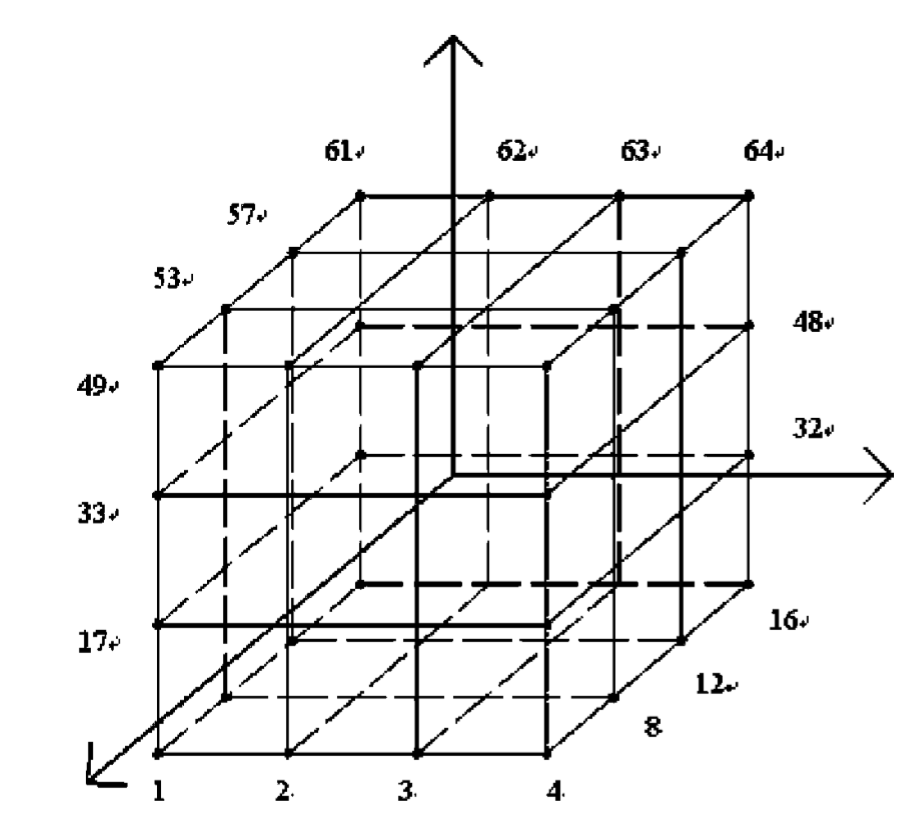
\includegraphics[width=0.75\textwidth]{Logos/VoxelEdges.PNG}
\caption{Darstellung der lokalen 4x4x4 Nachbarschaft} 
\label{fig:nachbarschaft} 
\end{figure}
\todo{richtig Bild zitieren}

Die Funktionen für die Intensitätswerte wird im Paper mit:
\begin{equation}
	f(x,y,z) = Ax^{2}+By^{2}+Cz^{2}+2Fyz+2Gzx+2Hxy+2Ix+2Jy+2Kz+D
\end{equation}
approximiert. Da der Gradient die Ableitung der Intensitätsfunktion ist, erhält man den dreidimensionalen Gradientenvektor $n$, indem die Funktion ableitetet wird:
\begin{equation}
	n = (Ax+Gz+Hy+I, By+Fz+Hx+J, Cz + Fy + Gx + K)
\end{equation}
Um den Gradienten zu Berechnen müssen die Parameter $A,B,C,E,F,G,H,I,J,K$  berechnet werden. Dies geschieht mithilfe der Methode der kleinsten Quadrate.
\todo{Methode der kleinsten Quadrate genauer beschreiben}

\subsection{LH-Werte}

Als nächster Schritt, nach der Kalkulation der Gradienten, folgt die Berechnung der Low- und High-Werte. Dazu wird in Richtung der Gradienten integriert. Hierfür wurde, wie auch von Nguyen, Heun's Methode, eine modifizierte Euler Methode, verwendet. Die für die Integration benutzte Formel lautet:
\begin{equation}
	u_{i+1} = u_{i} + \frac{1}{2}d(\triangledown f (u_{i}) + \triangledown f(u_{i}+d \triangledown f(u_{i}))) 
\end{equation}
Hierbei sind $u_{i}$ und $u_{i+1}$ die Positionen des aktuellen, beziehungsweise des nächsten Voxels. $\triangledown f(x)$ beschreibt den normalisierten Gradienten für die High-Werte und den normalisierten inversen Gradienten für die Low-Werte an Stelle $x$ . $d$ steht für die Schrittweite, die in dieser Arbeit auf einen Voxel festgelegt wurde.
Die Integration stoppt, wenn eine lokale Extremstelle oder ein Wendepunkt erreicht wird. Dies ist daran zu erkennen, dass die Länge des Gradienten an dieser Stelle null ist. Bei MRT-Daten muss ein Grenzwert festgelegt werden, da Gradienten nie null werden. Bei CT-Daten ist dies jedoch kein Problem. Wird ein solcher Punkt erreicht, wird der Intensitätswert dieses Voxels als Ergebnis für den Low- beziehungsweise High-Wert des Startvoxel gespeichert.
\newline
Anschließend wird ein LH-Histogramm mit allen berechneten LH-Wertpaaren erstellt. Hierbei sind auf der x-Achse die Low-Werte und auf der y-Achse die High-Werte angesiedelt. Die Werte der Achsen reichen von null bis zum jeweiligen Maximum des Low- beziehungsweise High-Werte.

\subsection{LH-Clustering}

Als nächstes, wird der erste Clusteringschritt berechnet. Dieser findet im LH-Raum statt, genauer wird er auf dem eben berechneten LH-Histogramm angewendet. Dabei kommt \textit{Meanshiftclustering} zum Einsatz. Der Ablauf davon geschieht wie folgt.
Vor dem Clustering muss eine Bandweite und ein Thresholdwert bestimmt werden, welche die Sensitivität des Clusterings festlegen. Die Bandweite liegt im Paper von Nguyen \cite{nguyen2012clustering} bei 7\% - 9\% des maximalen LH-Wertes und der Threshold bei 0,01. Anschließend kann das LH-Clustering auf jeden Punkt im Histogramm angewandt werden.
\newline
Für einen beliebigen Punkt, werden alle Punkte die innerhalb des Radius der Bandbreite liegen gespeichert. Diese Punkte bilden nun den gefundenen Cluster. Von diesem Cluster wird der neue Mittelpunkt, der jeweilige Mittelwert der beiden Koordinaten, berechnet. Um diesen Punkt wird erneut mit selben Radius alle Punkte die bisher nicht zu dem Cluster gehören gesucht und hinzugefügt. Dies geschieht solange, bis der Abstand des neu kalkulierte Mittelpunkt zum alten weniger als der Thresholdwert multipliziert mit die Bandweite ist. 
Nachdem dieses Prozedere für jeden Punkt im Histogramm ausgeführt wird, gibt es viele verschiedene Cluster. In einem nächsten Schritt, werden alle Cluster die sehr nah beieinander liegen verschmolzen. Dies betrifft jene Cluster, deren Mittelpunkte eine Distanz kleiner als die Hälfte der Bandweite zueinander haben.

\subsection{Räumliches-Clustering}

Als letzten Schritt, wird erneut auf jedem eben entstandenen Cluster \textit{Meanshiftclustering} angewendet. Dabei wird auf jedem Cluster einzeln und unabhängig von den anderen Clustern geclustert. Außerdem werden diesmal die räumlichen Informationen der Punkte in Betracht gezogen. Hierzu müssen zunächst erneut die beiden Parameter Bandweite und Threshold definiert werden. Das Clustering läuft wie zuvor im LH-Raum ab, nur wird statt im zweidimensionalem Raum mit einem zweidimensionalem Kreis im dreidimensionalem Raum des Volumens mit einer dreidimensionalen Kugel geclustert. Des Weiteren findet am Ende der Berechnung der Cluster keine Verschmelzung statt, da dies den Sinn der beiden verschiedenen Clusteringschritte zerstören würde. In den finalen Cluster haben alle Punkte jeweils ähnliche LH-Werte und liegen im Volumen nah beieinander. Würde man diese Cluster anhand ihrer räumlichen Informationen verschmelzen, haben die Punkte keine ähnlichen LH-Werte mehr und der erste Clusteringschritt wäre umsonst gewesen.







Der vorgestellte dritte hierarchische Clusteringsschritt wurde in dieser Arbeit nicht angewendet. Dies geschah aus dem Grund, dass bei diesem immer die beiden Cluster die sich am nächsten sind verschmolzen werden. Dies ist für die Aufgabe das Ventrikelsystem hervorzuheben nicht zielführend, da dieses mitten im Gehirn neben sehr vielen andern Cluster liegt. Folglich würde es relativ schnell mit andern Clustern verschmolzen werden.


%% ==============================
\chapter{\iflanguage{ngerman}{Design}{Concept}}
\label{sec:concept}
%% ==============================


Nachdem im vorherigen Kapitel die verschieden Methoden die genutzt werden vorgestellt wurde, beschäftigt sich dieser Abschnitt mit dem Softwaredesign der Implementierung dieser Methoden.
\newline
Die Implementierung dieser Bachelorarbeit teilt sich dabei in zwei verschieden Programme auf. Zum einen den sogenannten \textit{VolumeRenderHelper}, der für das Laden, Umwandeln, Verarbeiten und Speichern der Volumendaten zuständig ist. Zum anderen das Unityprogramm \textit{VolumeRenderer}, welches zur Visualisierung der vom \textit{VolumeRenderHelper} erzeugten Daten dient. Diese beiden Programme existierten bereits vor dieser Arbeit und sind in Vorarbeiten des IPRs entstanden.
\newline
In dieser Bachelorarbeit wurde der \textit{VolumeRenderHelper} um die vorgestellte Transferfunktion erweitert und der \textit{VolumeRenderer} geringfügig angepasst. Da beide Programme in \textit{csharp} geschrieben sind, wurden auch der Code, der im Laufe dieser Bachelorarbeit entstand in \textit{csharp geschriebn}. Als Entwicklerumgebung wurde dementsprechend \textit{Visual Studio 2017} von Microsoft verwendet.
\newline
Die Beiden Programme werden im folgenden als Helper und Renderer bezeichnet. Weiterhin wurde ein Pythonskript \textit{PlotHelper} geschrieben, um LH-Histogramme anzuzeigen.

\todo{Christians Paper}

Anfangs liegen die CT-Daten der Volumen in mehreren Dateien als Schnittbilder im DICOM Format vor. Diese werden mithilfe der \textit{Medical Imaging Interaction Toolkit} (kurz: \textit{MITK}) \textit{Workbench} \cite{mitk} zu einer einzelnen Datei im .nrrd Format umgewandelt, da nur Volumen in diesem Format vom Helper eingelesen werden können.
\newline
\textit{MITK} ist ein kostenloses open-source System zur Entwicklung von medizinischer Bildverarbeitungssoftware und wurde vom Deutschen Krebsforschungszentrum entwickelt. Dessen \textit{Workbench} bietet zum einen, das eben vorgestellte Laden und Umwandeln von DICOM Dateien, zum anderen auch diverse Segmentierungstools.


Die Darstellung von Volumendaten ist über den Renderer in Unity möglich. Der Benutzer hat hierbei mehrere Möglichkeiten Eingaben über Parameterfelder oder durch Drücken von Tasten zu machen und mit der Visualisierung zu interagieren. Zunächst muss er jedoch in das Parameterfeld \textit{Binary Data} via drag and drop eine binäre Volumendatei ziehen. Anschließend kann die Visualisierung gestartet werden. Hierbei hat der Nutzer die Möglichkeit die Kamera mit den Tasten $W$ $A$ $S$ $D$ zu bewegen als auch mit den seitlichen Pfeiltasten sowie der $Q$ und $E$ Taste das Volumen um verschiedene Achsen zu drehen. Die Position der Kamera sowie die Drehung des Volumens, kann ebenfalls durch verschiedene Parameterfeldern verändert werden.
\newline
Die Volumen, werden als Graubilder dargestellt, wobei die Helligkeit der einzelnen Voxel abhängig vom Intensitätswert bestimmt wird. Dabei kann der User über ein weiteres Parameterfeld entscheiden ob der Größte, der Kleinste, der Erste oder die Summe aller gefunden Voxel als Wert für die Farbgebung benutzt wird. Die Einstellung bei der der maximale wert genommen wird ist hierbei der Standard. Des Weiteren kann der Nutzer einen Threshold setzen, bei dem alle Voxel die eine Intensitätswert niedriger als diesen haben ignoriert werden.
\newline
Es existieren noch deutlich mehr Eingabefelder, mit denen der Benutzer die Darstellung des Volumens verändern und anpassen kann. Diese werden jedoch, da sie im Kontext dieser Bachelorarbeit nicht von Interesse sind, nicht alle vorgestellt.
\todo{evtl. raycasting}


\begin{figure}
\centering
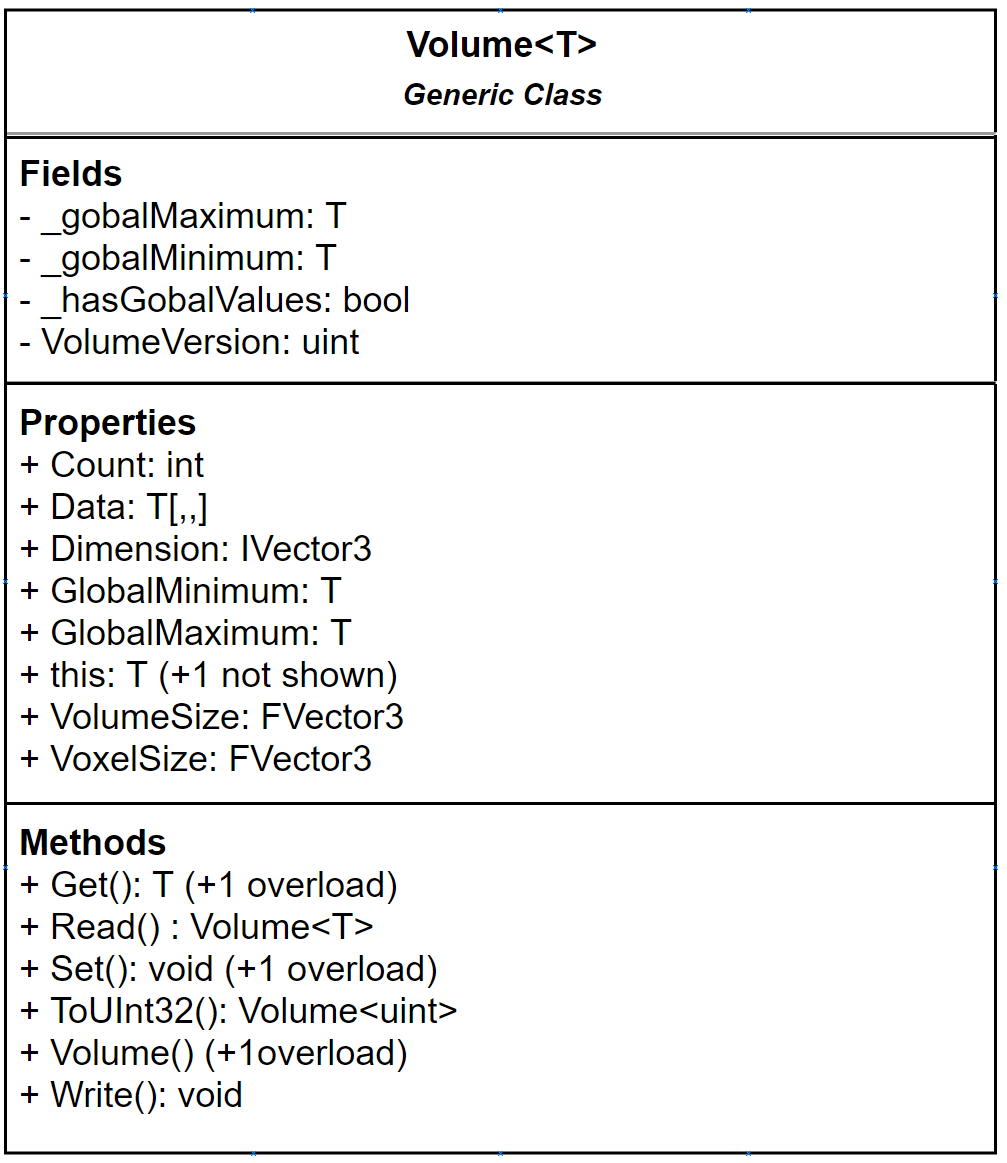
\includegraphics[width=0.6\textwidth]{Logos/Volume_UML.PNG}
\caption{UML-Diagramm des Volumens} 
\label{fig:volume_uml} 
\end{figure}


Die interne Speicherung des Volumens wird mit der generischen Klasse \textit{Volume} umgesetzt, deren Felder, Attribute und Methoden in \autoref{fig:volume_uml} zu sehen sind. Diese besitzt ein dreidimensionalen Array vom angegebenen generischen Datentyp, sowie Informationen über das Volumen, wie zum Beispiel Größe der Voxel oder Anzahl der Elemente pro Achse. Des Weiteren bietet die Klasse verschieden Funktionen um Informationen auszulesen oder zu bearbeiten. Zur Darstellung von dreidimensionale Koordinaten, werden die Klassen \textit{IVector3} und \textit{FVector3} benutzt. Diese stellen Vektoren dar, die entweder Integer, Ganzzahlen, oder Float, Dezimalzahlen, als $x,y$ und $z$ Werte speichern.


Die Interaktion des Benutzers mit dem Helper findet über eine Kommandozeile statt. Hierbei hat der Anwender die Befehle \textit{Load}, \textit{Dump}, \textit{Resample}, \textit{Info}, \textit{Write}, \textit{LHHistogram}, \textit{ClusterVolume} und \textit{MergeCluster} zur Auswahl. Dies ist im UML-Diagramm in \autoref{fig:modul_uml} zu sehen. Jedes Modul hat dabei seine eigene Syntax die mithilfe eines Help Befehls angezeigt werden kann.


\begin{figure}
\centering 
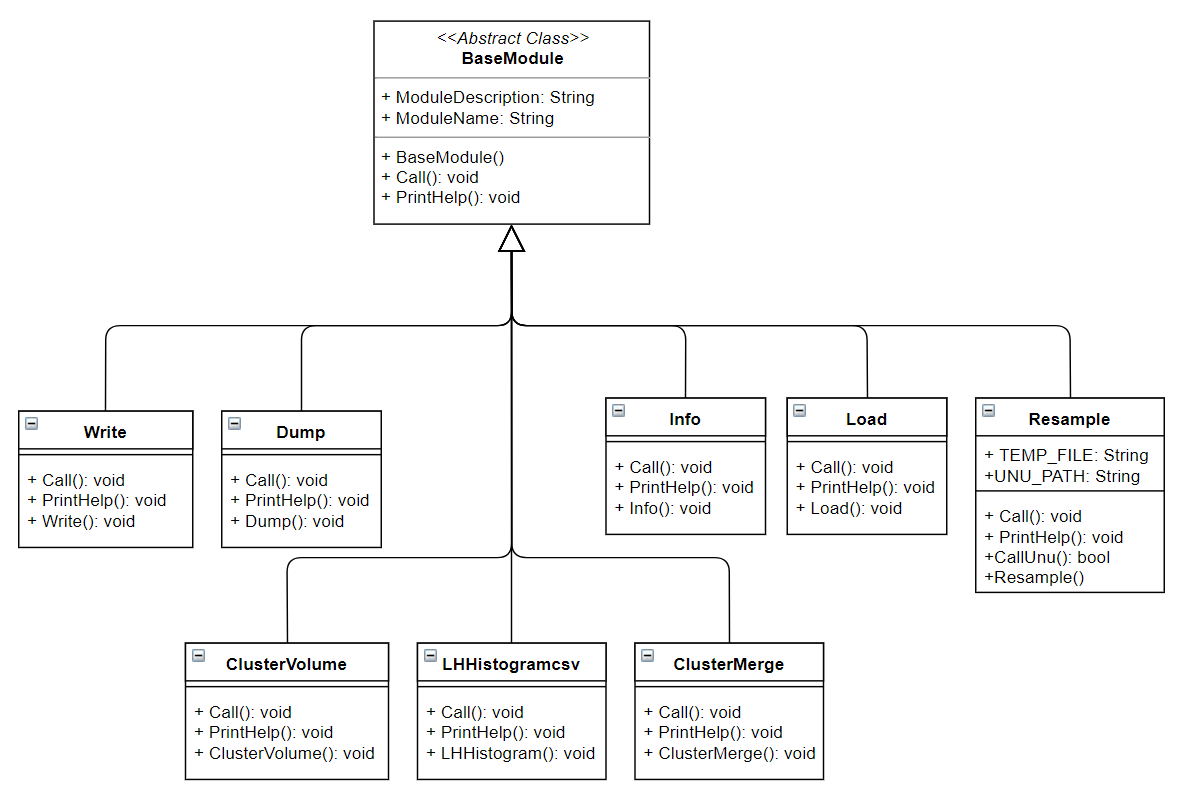
\includegraphics[width=\textwidth]{Logos/Modules_UML.PNG}
\caption{UML-Diagramm über die Module} 
\label{fig:modul_uml} 
\end{figure}


Die Funktionen der Module entsprechen deren Namen. So lädt \textit{Load} bespielsweise eine .nrrd oder binäre Datei, \textit{Dump} und \textit{Write} speichern das geladene Volumen als binäre oder .nrrd Datei ab, \textit{Info} gibt Informationen über das aktuell geladene Volumen zurück und \textit{Resample} lässt den Anwender die Größe des Volumens verändern.
\newline
Wird der \textit{Dump} Befehl mit einem $u$ am Ende aufgerufen, so wird das Volumen vor dem Speichern zum Typ $unsigned$ $int$ gecastet. Dies geschieht indem auf alle Werte der Betrag des minimalen Wertes aufaddiert wird. Dadurch verschieben sich die Werte so, dass das Minimum bei null liegt, also nur noch positive Zahlen im Volumen vorhanden sind. Dies ist für die Darstellung im Renderer wichtig, da dieser nur mit positiven Zahlen funktioniert. Des Weiteren müssen alle binären Dateien mit dem Suffix .bin.txt gespeichert werden, da Unity die Dateien sonst nicht einlesen kann.


Im Folgenden werden hauptsächlich die Module \textit{LHHistogram}, \textit{ClusterVolume} und \textit{MergeCluster} erläutert, da diese im Laufe dieser Arbeit entstanden sind. \textit{LHHistogram} berechnet das LH-Histogramm des geladenen Volumens und speichert dieses in einer .csv Datei ab. \textit{ClusterVolume} kalkuliert ebenfalls die LH-Werte des Volumens, führt jedoch hinterher noch die beiden Clusteringsschritte des Verfahrens aus. Als Ausgabe speichert das Modul eine binäre Datei eines Volumens, in welchem die verschiedenen IDs der Cluster gespeichert sind. Die Idee dahinter wird im laufe diese Kapitels erklärt. Das Modul \textit{MergeCluster} dient der Verschmelzung der gewünschten IDs mit dem ursprünglichen Volumen. Das Ergebnis dessen, ist eine finale binäre Datei, die im Renderer das Ventrikelsystem visualisiert. Ein Überblick über den gesamten Aufbau und Ablauf der Implementierung ist in  \autoref{fig:ueberblick} zu sehen.

\begin{figure}
\centering 
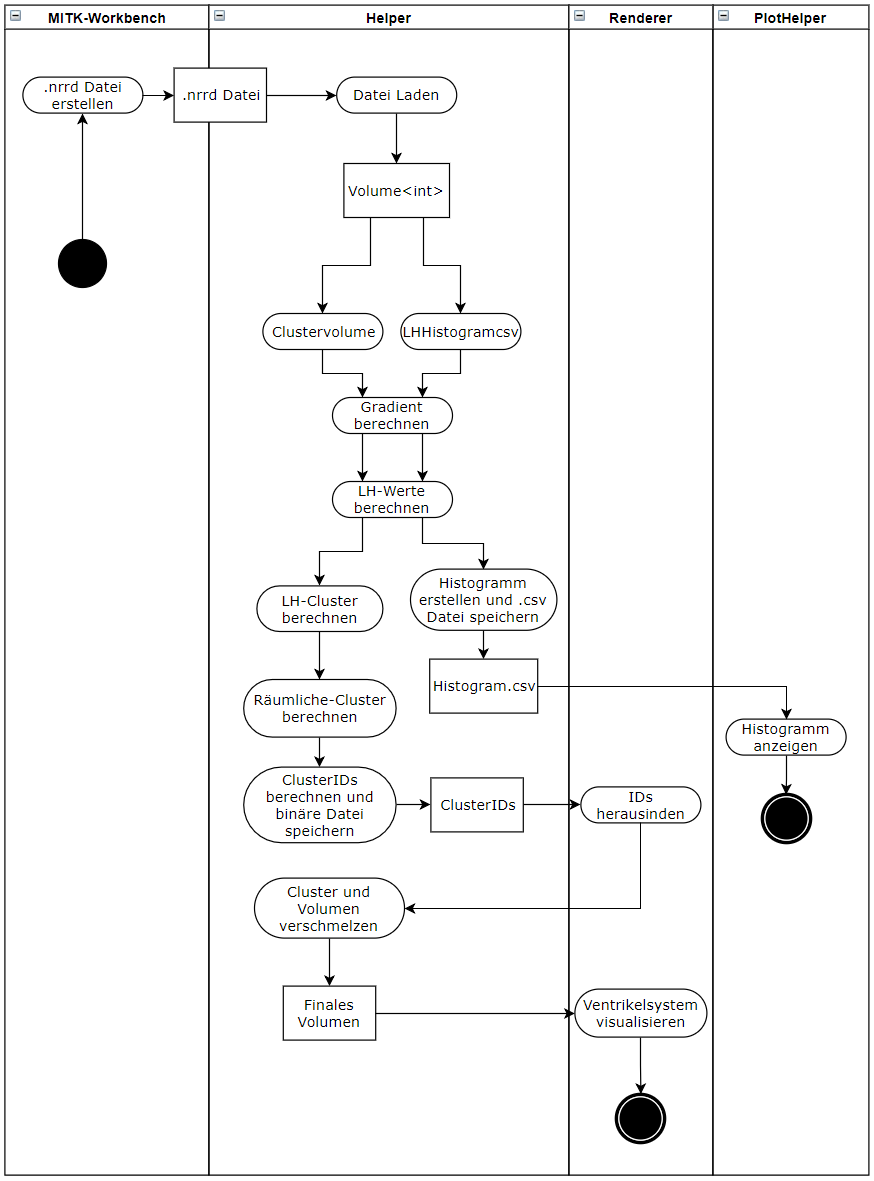
\includegraphics[width=\textwidth]{Logos/Ueberblick2.png}
\caption{Überblick über den Ablauf} 
\label{fig:ueberblick} 
\end{figure}


Der Ablauf der Berechnung startet in der statischen \textit{Gradient} Klasse. Diese ist eine Implementierung des Verfahren von Hong \cite{hong2003method}. Zur Berechnung wird der Funktion \textit{CalcGradientVolume} das Volumen der Intensitätswerte, als Volumen aus Integern, als Parameter übergeben. Wie im vorherigen Kapitel besprochen, können die Gradienten nicht für einen Voxel direkt berechnet werden, sondern nur für die Punkte zwischen den Voxeln. Aus diesem Grund ist das Ergebnisvolumen um ein Voxel in jeder Achse kleiner als das Volumen der Intensitätswerte. In \autoref{fig:shift} ist ein zweidimensionales Beispiel zu sehen, bei dem die Gradienten berechnet werden und die Dimension der Achsen dadurch um eins kleiner wird. Die Dimension der Intensitätswerte ist ein 5x5 Gitter, in der Abbildung in schwarz zu sehen. Nachdem die Gradienten immer zwischen 4 Punkten berechnet wurde, ist zu sehen, dass die Dimension der Gradienten ein 4x4 Gitter ist. In der Abbildung in rot zu sehen. Als Ergebnis der  \textit{CalcGradientVolume} Funktion wird ein Volumen vom Typen \textit{FVector3} zurückgegeben.


\begin{figure}
\centering 
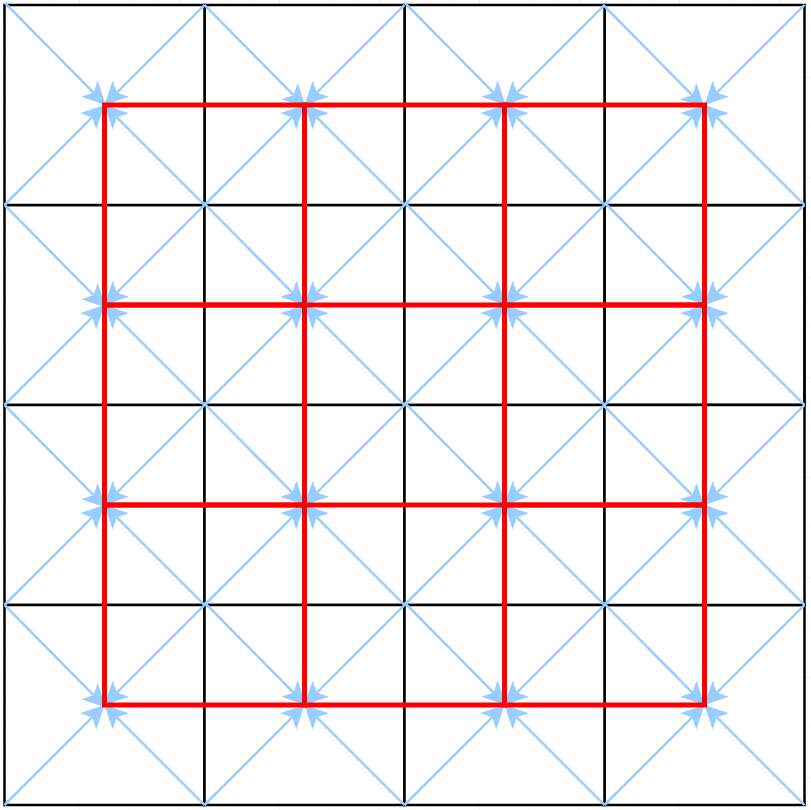
\includegraphics[width=0.75\textwidth]{Logos/VoxelShift.png}
\caption{2D Beispiel warum das Volumen kleiner wird} 
\label{fig:shift} 
\end{figure}



Die Berechnung der LH-Werte findet in der statischen Klasse \textit{LHValues} in der Funktion \textit{LHValueVolume} statt. Als Parameter wird das \textit{FVector3} Volumen der Gradienten aus dem Schritt davor entgegengenommen. Da für die Berechnung der LH-Werte die Intensitätswerte und die Gradienten am gleichen Punkt vorhanden seien müssen, müssen die Intensitätswerte für das verschobene Volumen der Gradienten berechnet werden. Dazu wurde eine einfache Interpolation durchgeführt, indem von allen 8 Nachbarn eines Punktes die Intensitätswerte aufaddiert und hinterher durch acht geteilt wurden. Hierbei muss jedoch beachtet werden, dass die Werte dadurch verändert werden, und Informationen verloren gehen.


Hat der Benutzer das Modul \textit{LHHistogram} aufgerufen, wird im Anschluss das LH-Histogramm in der Klasse \textit{LHHistogramCSV} erstellt und wird von ihr als .csv Datei in einem vom Anwender angegebenen Pfad abgespeichert.
\newline
An dieser Stelle kommt das Pythonskript \textit{PlotHelper} zum Einsatz. Dieses lädt die .csv Datei und visualisiert das LH-Histogramm mithilfe einer kalt-zu-heiß-Farbrampe in einem zweidimensionalem Koordinatensystem.
\newline
Hierbei ist zu beachten, dass das Histogramm abhängig von der Häufigkeit des Vorkommens eines LH-Wertpaares im Volumen gebildet wird. Diese werden im jeweils dazu passenden Kästchen des Koordinatensystems gespeichert. Dies ist ein simplerer Vorgehen, als das im Paper von Nguyen \cite{nguyen2012clustering} benutzte Erstellen des Histogramms abhängig von einer für jeden Voxel berechneten Gewichtung. Da die Arbeit an der Implementierung zeitlich beschränkt war, wurde diese Gewichtung, die einzig und allein einer genaueren Darstellung des für das Verfahren irrelevante LH-Histogramm dient, vernachlässigt. Die Gewichtung ist für das Clustering belanglos, da dort ein Histogramm wie oben beschrieben, abhängig von der Häufigkeit der LH-Werte verwendet wird.
\newline
Bei der Erstellung des Histogramms im \textit{LHHistogram} Modul wird weiterhin der Logarithmus der Anzahl der Einträge jedes Kästchens genommen. Dies geschieht aus dem Grund der großen Diskrepanz zwischen der Anzahl der Einträge an den meisten Stellen im Histogramm im Vergleich zu dem Maximum. Dies lässt bei der Darstellung mit einer Farbrampe fast alles mit der Farbe des Minimums anzeigen. Da die Logarithmusfunktion für schnell wachsende Zahlen nur sehr langsam steigt, eignet sie sich dafür, diesen großen Unterschied anzupassen.


Wurde jedoch das \textit{ClusterVolume} Modul aufgerufen, wird mit den beiden Clusteringschritten fortgefahren.
\newline
Die Berechnung der LH-Cluster, die in der \textit{LHClustering} Klasse geschieht, nimmt das Volumen mit den LH-Werten entgegen und rechnet dieses aus Performancegründen, wie oben beschrieben, in ein ein Histogramm um. Dieser Schritt könnte gespart werden, wenn die Methode \textit{LHValueVolume} direkt ein Histogramm als Rückgabewert liefern würde. Dies würde auch das \textit{LHHistogram} Modul verbessern, da damit die Umrechnung in dieser Klasse ebenso hinfällig wird. Als Ergebnis der Clusteringfunktion \textit{ComputeLHClusters} wird eine Liste der Cluster zurückgegeben, wobei ein Cluster aus einer Liste von \textit{IVector3} besteht. Die Cluster werden nur als Liste der räumliche Informationen der Voxel gespeichert, da für den nächsten Clusteringschritt  lediglich diese Information benötigt wird. 


Anschließend geht es in der \textit{SpatialClustering} Klasse mit der Berechnung der räumlichen Cluster weiter. Diese werden aus dem Grund, dass wieder \textit{Meanshiftclustering} verwendet wird, mit einer ähnlichen Implementierung wie in der \textit{LHClustering} Klasse kalkuliert. Diesmal wird jedoch nicht auf einem Histogramm, sondern direkt auf den übergebenen Listen die Berechnung durchgeführt. Folglich muss für jede Iteration eines Mittelpunktes die gesamte Liste durch iteriert werden.
\newline
Als Ergebnis wird erneut eine Liste von Listen vom Typ \textit{IVector3} zurückgegeben.


Nachdem alle Cluster kalkuliert wurden, werden sie in einem Volumen gespeichert. Jeder Cluster bekommt dabei zunächst seine eigene ID beginnend bei eins. Das Volumen wird dann mit den verschiedenen IDs gefüllt. Dies geschieht indem für jeden Cluster an den Positionen der Punkte die jeweilige ID gespeichert wird. Alle anderen Voxel des Clustervolumen wird der Wert null zugewiesen. Dieses Volumen wird als binäre Datei gespeichert und ist das Ergebnis der ClusterVolume Moduls. Es ist bei diesem Modul sehr wichtig, dass es, wie es bei dem \textit{Dump} Befehl möglich ist, mit einem $u$ am Ende aufgerufen wird, da das Ergebnis sonst nicht vom Renderer dargestellt werden kann.


Das Ergebnis muss anschließend vom Nutzer in Unity geladen werden.
\newline
Hierbei kommt die von dieser Arbeit vorgenommenen Anpassung am Renderer zum Einsatz. Dadurch ist es dem Benutzer möglich über ein Eingabefeld während der Visualisierung einen Wert, oder einen Wertebereich anzugeben. Dieser wird dann in einer gewählten Farbe, standardmäßig rot, hervorgehoben. Dies muss der Anwender nutzen, um die IDs, die das Ventrikelsystem beschreiben, zu finden.


Hat er dies getan kann er mit dem\textit{MergeCluster} Modul des Helpers das Ergebnis zusammenfügen und die finale Visualisierung erhalten. Beim Aufruf muss der Nutzer das Intensitätsvolumen, das Clustervolumen mit den IDs und die ausgewählten IDs als Parameter übergeben. Anschließend wird an den Stellen der ClusterIDs die Werte im Intensitäsvolumen mit dem Wert 5000 überschrieben, da nach dem beschriebenen Werteshift ins positive der maximale Intensitätswert bei ungefähr 4500 liegt. Dies erhöht das Maximum des Volumens nur gering und lässt es zu die zu visualisierenden Bereiche klar vom Rest abzugrenzen. Dieses Volumen wird erneut als binäre Datei gespeichert.
\newline
Als letzten Schritt kann der Benutzer die finale binäre Datei in Unity laden. Stellt er den Wert der eben erklärten Erweiterung des Renderer auf 5000, wird das Ventrikelsystem in den ursprünglichen Volumendaten rot hervorgehoben.














































%% ==============================
\chapter{\iflanguage{ngerman}{Implementierung}{Implementation}}
\label{sec:implementation}
%% ==============================




Nachdem im letzten Kapitel das Softwaredesign besprochen wurde, beschäftigt sich das Kommende mit der Implementierung an sich.


Es ergaben sich bei der Implementierung verschiedene Probleme. Beispielsweise wurde anfangs das Verfahren mit MRT-Daten getestet. Dies war von wenig Erfolg, da die Volumendaten große Unterschiede zu den CT-Daten aufweisen und somit das Verfahren nicht funktionierte.


Die vorgestellten Module erben alle von der abstrakten \textit{BaseModule} Klasse, die es ihnen vorschreibt, eine \textit{Call} sowie eine \textit{PrintHelp} Methode zu implementieren.
\newline
Ruft der Benutzer ein Modul des Helpers über den jeweiligen Befehl in der Konsole auf, so wird die jeweilige \textit{Call} Methode, mit denen vom Benutzer gegebenen Parameter, ausgeführt.
\newline
Es existiert für jeden der Berechnungsschritte der Gradienten, LH-Werte, LH-Cluster und Räumlichen-Cluster eine eigene statische Klasse, die eine öffentliche Methode besitzt. Diese berechnet für die gegebenen Parameter den jeweiligen Schritt und gibt das Ergebnis zurück. 
\newline
Beispielsweise wird in der \textit{Call} Methode des \textit{LHHistogram} Moduls, zuerst die \textit{CalcGradientVolume} Funktion der \textit{Gradient} Klasse mit dem Intensitätsvolumen als Parameter aufgerufen. Danach wird die \textit{LHValuesVolume} Methode der \textit{LHValues} Klasse mit dem Ergebnis der vorherigen Funktion als Parameter ausgeführt. Aus dessen Ergebnis wird in der \textit{Call} Methode des Moduls direkt das LH-Histogramm erstellt und gespeichert. Im Modul \textit{ClusterVolume} läuft die Berechnung ebenso über das Aufrufen von den Methoden der jeweiligen Klassen ab.
\newline
Das Modul \textit{MergeCluster} führt seine Berechnung komplett in der \textit{Call} Funktion, da die Kalkulation nicht sehr aufwändig ist, aus.
\newline
Die Implementierung der Klassen und deren Methoden ist das Thema dieses Kapitels und wird im Folgenden genauer erläutert.
\newline
Bei der  Kalkulation der Gradienten wird parallel über jeden Voxel im Intensitätsvolumen iteriert und für jeden die Implementierung von Hong's Methode \cite{} aufgerufen.
\newline
Für die Berechnung der Methode wird eine Gewichtung und die Koordinaten aller 64 Punkte im Koordinatensystem der lokalen Nachbarschaft benötigt. Da das gesamte Volumen die selbe Voxellänge hat und die Koordinaten in der lokalen Nachbarschaft immer gleich sind, können diese beiden Werte für alle 64 Nachbarn einmalig in einem Vorverarbeitungsschritt berechnet werden. Sie werden dabei in einem 64 Elemente großes Array, mit der gleichen Nummerierung wie in \autoref{fig:nachbarschaft} gezeigt, gespeichert. Bei der Kalkulation jedes Gradienten müssen lediglich die beiden Arrays durch iteriert werden um die entsprechenden Gewichtung und Koordinate  des Nachbars zu erhalten


\begin{figure}[!h] 
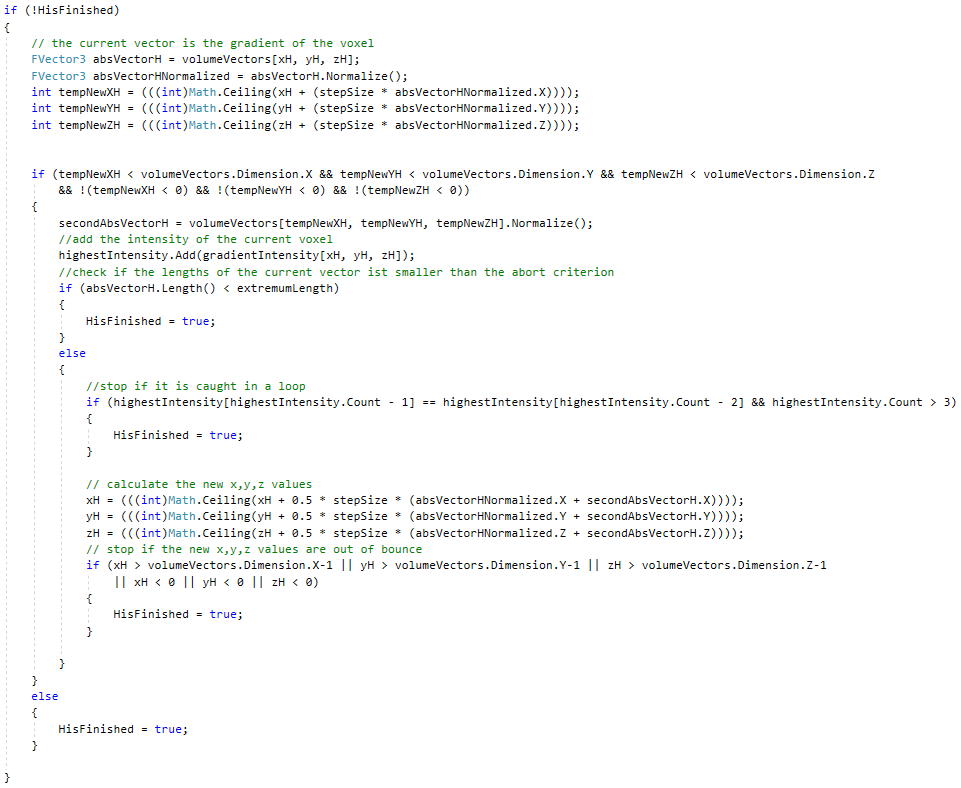
\includegraphics[width=1.2\textwidth]{Logos/LH_Code.PNG}
\caption{Implementierung der Berechnung der High-Werte} 
\label{fig:lh_code} 
\end{figure}


In \autoref{fig:lh_code} kann man den Code zur Berechnung der High-Werte sehen. Der Code liegt innerhalb einer while-Schleife, die so lange aufgerufen wird, bis die Berechnung des Low- und des High-Wertes abgeschlossen, also \textit{LisFinished} und \textit{HisFinished} true sind. Die Berechnung des Low-Wertes ist ebenfalls in der Schleife und sieht bis auf die Richtung der neuen \textit{absVector} und \textit{secondAbsVector} gleich aus. Folglich sind alle hier gegebenen Erklärung und Anmerkungen ebenso auf die Berechnung der Low-Werte zu beziehen.
\newline
Am Anfang eines Durchlaufes wird der normalisierte Gradienten des aktuellen Punktes in \textit{absVectorNormalized} gespeichert. Anschließend wird der Punkt des zweiten normalisierten Vektors berechnet. Liegt dieser außerhalb des Volumens, so wird die Integration beendet. Liegt er jedoch innerhalb des Volumens, so wird der \textit{secondAbsVector} ausgelesen und der Intensitätswert des aktuellen Punktes zu der Liste \textit{highestIntensity} hinzugefügt. Ist der Gradient des aktuellen Punktes kleiner als die \textit{extremumLength}, welche im Falle von CT-Daten bei null liegt, wird die Integration beendet.
\newline
Andernfalls wird zunächst mithilfe der \textit{highestIntensity} Liste nach Schleifen gesucht. Bei sehr kleinen Gradienten, die jedoch größer als null sind, kann es vorkommen, dass das Verfahren immer wieder den selben Punkt findet und somit in einer Endlosschleife feststeckt. Wie in \autoref{fig:lh_code]} zu sehen ist, wird dabei jedoch erst getestet ob die Liste schon mehr als 3 Einträge hat. Dies geschieht aus dem Grund, dass anfangs, vor der while-Schleife bereits der Intensitätswert des Startvoxels zur Liste hinzugefügt werden muss. Dies geschieht aus dem Grund, dass sonst, würde das Verfahren bei dem ersten Abbruchkriterium bei der ersten Iteration schon stoppen, die \textit{highestIntensity} Liste leer wäre, und es kein Ergebnis für den High-Wert gäbe. Diese Kontrolle könnte jedoch über die Koordinaten der iterierten Punkte geschehen, um dem unwahrscheinlichem Fall, dass zwei durch die Integration hintereinander besuchte Punkte genau den selben Intensitätswert haben.
\newline
Anschließend wird der nächste Punkt der Integration mithilfe von \textit{absVectorNormalized} und \textit{secondAbsVecotr} gemäß Heun's Methode, die im Kapitel der Methode vorgestellt wurde, ermittelt. Erneut endet die Integration, falls der neu berechnete Punkt außerhalb des Volumens liegt.
\newline
Dieser Vorgang wiederholt sich für den High- als auch für den Low-Wert solange, bis die Integration aus einem der gegebenen Abbruchkriterien stoppt. In diesem Fall wird der letzte Eintrag der \textit{highestIntensity} Liste ausgelesen und als Ergebnis für den High-Wert gespeichert. Ebenso passiert dies mit der für die Low-Werte äquivalenten \textit{lowestIntensity} Liste.
\newline
Der Fall, dass ein Iterationsschritt in einer der gezeigten Formen außerhalb des Volumens liegt, und deshalb das Verfahren gestoppt wird, kommt in ungefähr 2-\%-3\% der Fälle vor. Des Weiteren kommt es bei zirka 25\% aller Berechnung dazu, dass die LH-Werte vertauscht waren, also der Low- größer als der High-Wert war. Dem wird entgegengewirkt, indem bei einem Vorkommen dieses Problems die beiden Werte vertauscht gespeichert werden. Es war noch nicht möglich den Grund für diese Verwechslung herauszufinden.


Die Implementierung des LH-Clusterings wurde mit einer parallelen for-Schleife realisiert, die über die L-Werte mit der Schrittweite von 5 iteriert. Für jede Spalte i wird dann die in \autoref{alg:clustering} beschriebene Funktion aufgerufen.
\newline
Die erste for-Schleife iteriert über die H-Werte. Der Parameter j beginnt mit dem Wert i und wird, wie dieser, mit der Schrittweite 5 hochgezählt. Dies hat den Grund, dass es im LH-Histogramm keine Einträge gibt, bei denen der Low- höher als der High-Wert ist. Alle durch die beiden Schleifen entstehenden Punkte $(i, j)$ sind jeweils die Startpunkte einer Clustersuche.
\newline
Um nicht zu viele Cluster zwischenspeichern zu müssen und erst ganz am Ende alle ähnlichen Cluster zu verschmelzen, werden bereits am Ende jeder Spalte deren Ergebniscluster soweit wie möglich verschmolzen.
\newline
Weiterhin speichert der temporäre Cluster \textit{AktuellerCluster} lediglich die Koordinaten der zum Cluster dazugehörigen Punkte im Histogramm, jedoch nicht die räumlichen Informationen der darin gespeicherten Voxel, ab. Erst am Ende der parallelen Schleife, wenn alle Ergebnisse gesammelt und die Cluster verschmolzen wurden, werden diese Daten ausgelesen. Dies spart Speicherplatz und Berechnungszeit, da in einem einzigen Kästchen im LH-Histogramm mehrere Tausend Voxel gespeichert sein können.


\IncMargin{1em}
\begin{algorithm}
\SetKwData{Left}{left}\SetKwData{This}{this}\SetKwData{Up}{up}
\SetKwFunction{Union}{Union}\SetKwFunction{FindCompress}{FindCompress}
\SetKwInOut{Input}{input}\SetKwInOut{Output}{output}

 \Input{LH-Histogramm, Spalte i}
 \Output{LH-Clusters}
 \BlankLine
 $AlleErgbnisCluster$\;
 $Mittelpunkt$\;
 $AlterMittelpunkt$\;
 $AktuellerCluster$\;
 \For{$j\leftarrow i$ \KwTo Rand des Histogramms, Schrittweite: 5}{
  $Mittelpunkt \leftarrow (i,j)$\;
 \While{Abstand(NeuerMittelpunkt, AlterMittelpunkt) > Threshold * Bandweite}{
  \For{$(k, l)\leftarrow$ Alle Punkte im Radius der Bandweite um den Mittelpunkt}{
      \If{NochNichtTeilDesClusters((k, l))}{
	$AktuellerCluster.Hinzufuegen((k, l))$\;
     }
    }
   $AlterMittelpunkt \leftarrow Mittelpunkt$\;
    $Mittelpunkt \leftarrow NeuenMittelpunktBerechnen(AktuellerCluster)$\;
  }
  $AlleErgebnisCluster.Hinzufügen(AktuellerCluster)$\;
 $ Leeren(AktuellerCluster)$\;
 }
$VerschmelzeNaheCluster(AlleErgebnisCluster)$\;
$return$ $AlleErgebnisCluste$r\;

 \caption{Pseudocode der Implementierung der LH-Cluster}
 \label{alg:clustering}
\end{algorithm}\DecMargin{1em}


Das LH-Clustering wurde anfangs wie im Paper von Nguyen \cite{nguyen2012clustering} über das gesamte Histogramm mit einer Bandweite von 7\% des maximalen LH-Wertes für jeden Kasten berechnet. Dies ist aus mehreren Gründen schlecht. Zum einen ist der maximale LH-Wert sehr hoch, über 4000, obwohl in etwa nur 0,3\% Voxel einen Wert von über 2400 haben. Zum anderen liegen über 5\% der LH-Werte unter 5. Die Kombination aus diesen Gründen, machte das Clustering extrem langsam. Im Bereich von 0 bis 50  wurde in einem sehr großen Radius geclustert, wodurch mit jeder Iteration sehe viele Cluster gefunden und hinzugefügt werden mussten.
\newline
Eine erste Maßnahme um das Problem zu beheben, war es alle Low- und High- Werten, die über 2400 waren jeweils auf 2400 zu setzten. Dadurch wurden nur wenige Werte verändert und der Clusteringradius wurde deutlich kleiner. Dies konnte das beschriebene Problem jedoch nicht alleine lösen, da immer noch viele Punkte gefunden und dies für jeden Kasten im Histogramm durchgeführt werden musste.
\newline
Also wurde als nächste Verbesserung eine Schrittweite beim Clustern eingeführt. Dies geschah aus der Beobachtung heraus, dass zwei bis drei oder eventuell sogar mehr direkt nebeneinanderliegende Kasten meist zum selben oder einen so ähnlichen Cluster führen, dass diese im letzten Schritt des Clusteringsverfahrens verschmolzen wurden. Diese Änderung verbesserte die Berechnungszeit erneut, jedoch  dauert die Berechnung immer noch relativ lange und es entstanden sehr viele Cluster. Diese durchzuschauen benötigte viel Zeit und das Gehirn wurde dabei meist als viele sehr große Cluster erkannt. Daraufhin wurde das Clustering auf einen LH-Wertbereich von 1025 bis 1075 begrenzt und die Bandweite auf 0,1\% des maximalen LH-Wertes gesetzt. Diese Änderung führte zum Erfolg und das Ventrikelsystem war innerhalb der paar hunderten Clustern mit ein bisschen Aufwand zu erkennen.
\newline
In der statischen Klasse \textit{SpatialClustering} ist die Implementierung zur Berechnung der räumlichen Cluster und dem Clustervolumen der IDs zu finden.
\newline
Die Kalkulation der räumlichen Clustern wurde dabei, wie die Berechnung der LH-Cluster, mit einer parallelen for-Schleife realisiert. Diese iteriert über die LH-Cluster und ruft für jeden Cluster die in \autoref{fig:spatclust_code} gezeigte Funktion auf. Die Cluster sind in der globalen Liste \textit{LHClusters} gespeichert. Sie haben den Typ einer Liste von \textit{IVector3}. 
\newline
Die Suche nach Clustern liegt in einer while-Schleife, die so lange ausgeführt wird, solange der LH-Cluster genug Elemente hat, damit ein Cluster mit der Mindestgröße an Elementen gefunden werden kann. 
\newline
Das Finden von Clustern läuft dabei folgendermaßen ab. Der erste Punkt im LH-Cluster wird als Startmittelpunkt gewählt. Danach wird durch alle Punkte iteriert und diejenigen die innerhalb der Bandweite liegen sowohl zum temporärem Cluster \textit{currentSpatialCluster} als auch zum HashSet der zu entfernenden Punkte \textit{toRemove} hinzugefügt. Anschließend werden, alle Elemente von \textit{toRemove} aus dem LH-Cluster entfernt und wie beim LH-Clustering auch ein neuer Mittelpunkt errechnet. Wenn das Abbruchkriterium der zwei naheliegenden aufeinanderfolgenden Mittelpunkte erfüllt ist, wird der temporäre Cluster \textit{currentSpatialCluster} zur Liste der Ergebniscluster \textit{resultClusters} hinzugefügt, falls er genug Elemente besitzt.
\newline
Für die Bandweite und die minimale Distanz für das Abbruchkriterium wurden im Paper von Nguyen \cite{} keine Werte angegeben. In dieser Bachelorarbeit wurde die Bandweite auf 15 und die Distanz auf 0,01 gesetzt. Diese Werte wurden durch Testen herausgefunden und führten zu den besten Ergebnissen.
\newline
Anschließend wird in der Funktion \textit{ComputeIDs}, der die Cluster als Parameter übergeben werden, das Clustervolumen erstellt und zurückgegeben.



\begin{figure}[!h] 
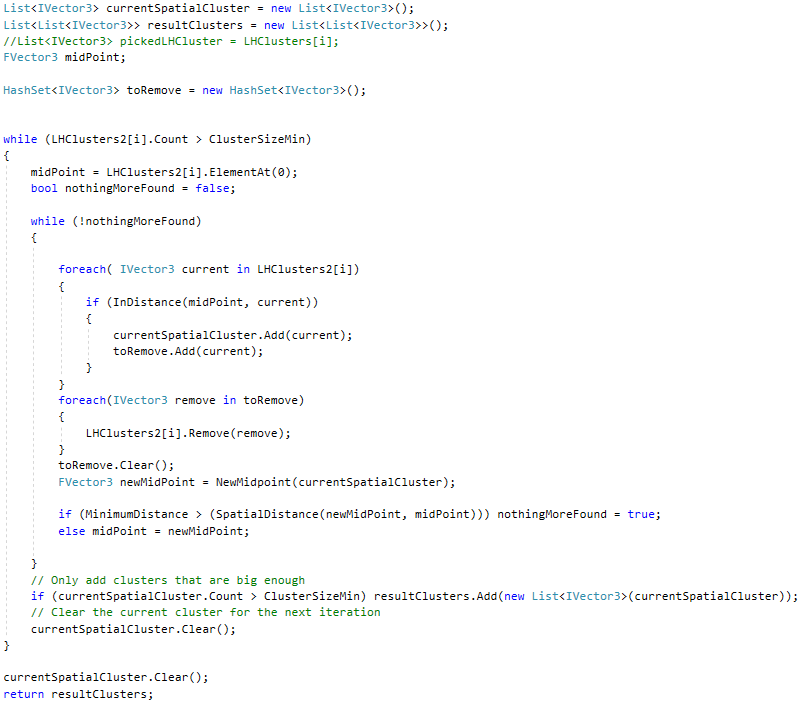
\includegraphics[width=1.2\textwidth]{Logos/Spatial_Code.PNG}
\caption{Implementierung der Berechnung der Gewichte und Koordinaten} 
\label{fig:spatclust_code} 
\end{figure}


Die Erweiterung die am Renderer vorgenommen wurden, wurden im Shader programmiert. Zuerst wurde eine drop-down-list hinzugefügt, über die der Nutzer zwischen den Modi \textit{Default}, \textit{SpecificValue} und \textit{SpecificValueRange} wählen konnte. Weiterhin wurden drei Textfelder hinzugefügt, über die es dem Anwender möglich ist den spezifischen Wert als auch den Wertebereich anzugeben. Des Weiteren wurde noch ein Farbfeld hinzugefügt, mit welchem die Farbe, in der hervorgehobenen Bereiche dargestellt wird, anzeigt wird und vom Benutzer verändert werden kann.
\newline
Der \textit{Default} Modus steht hierbei für die schon vorher dagewesene Implementierung der Farbgebung. Diese wurde weitestgehend in den beiden anderen beiden Modi übernommen. Der Unterschied besteht jedoch darin, dass wenn ein Voxel bei \textit{SpeicifcValue}mit dem spezifischen Wert, oder bei \textit{SpecificValueRange} innerhalb des Wertebereichs gefunden wird, dieser in der Farbe des Farbfeldes angezeigt wird. Alle andern Voxel bekommen die selbe Farbe, die sie auch im \textit{Default} Modus erhalten würden.
























































%% ==============================
\chapter{\iflanguage{ngerman}{Ergebnisse}{Results}}
\label{sec:results}
%% ==============================





Dieses Kapitel beschäftigt sich mit den Ergebnissen der Segmentierung, sowie mit der Evaluation des Verfahrens. Der Abschnitt teilt sich dabei folgendermaßen auf. Als erstes werden die Ergebnisse der Visualisierung des Ventrikelsystems gezeigt und evaluiert. Dabei wurde für die Auswertung ein Interview mit einem Arzt durchgeführt. Danach wird eine Nutzerstudie vorgestellt, die die Benutzerfreundlichkeit des Systems testet. Als letztes wird die Berechnungszeit der Implementierung besprochen.


\subsection{Visualisierung}

\subsubsection{Ventrikelsystem}

Bevor die Visualisierungen ausgewertet werden können, muss zunächst das Ventrikelsystem erläutert werden. In \autoref{fig:ventrik} ist das Ventrikelsystem zu sehen. Dieses besteht aus vier verschiedenen Ventrikeln. Zum einen der linke und der rechte Seitenventrikel, die oberen beiden Bögen, die in der Abbildung zu sehen sind. Zum anderen der dritte und vierte Ventrikel, die zwischen den beiden Seitenventrikeln liegen und nach unten weggehen. Die Seitenventrikel bestehen aus einem Vorderhorn, Nr. 1a,  einem Hinterhorn, Nr. 1b, und einem Unterhorn, Nr. 2. Der dritte Ventrikel ist mit der Nummer 3 und der vierte Ventrikel mit der Nummer 4 versehen. Bei der Ventrikelpunktion, wird einer der beiden Seitenventrikel im vorderen Bereich punktiert. Dies macht vor allem die Darstellung der Seitenventrikel relevant.

\begin{figure}[!h] 
\centering 
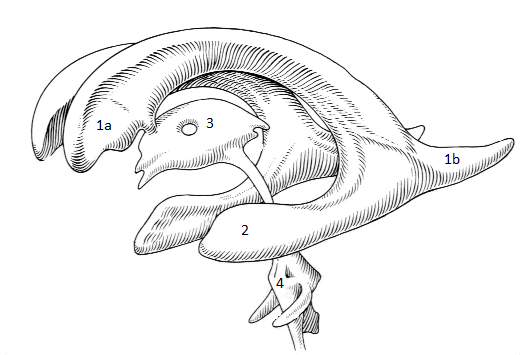
\includegraphics[width=0.75\textwidth]{Logos/Ventrikelsystem_V3.png}
\caption{Zeichnung des Ventrikelsystems  \\  Frei nach \protect\cite{ventrik}} 
\label{fig:ventrik} 
\end{figure}


\subsubsection{Visualisierungen}

Die in diesem Unterkapitel gezeigten Visualisierungen wurde alle auf Volumen mit einer Auflösung von 256x101x256 Pixeln berechnet. Aus dem Grund, dass dies ein gute Balance zwischen der Auflösung und der Berechnungszeit der Ergebnisse darstellt. Im Unterkapitel Berechnungszeit wird dies genauer beschrieben.
\newline
In \autoref{fig:norm1_s} und \autoref{fig:norm1_u} ist die Visualisierung des ersten normalen Ventrikelsystems, in \autoref{fig:norm2_s} und \autoref{fig:norm2_u} die Visualisierung des zweiten normalen Ventrikelsystems und schließlich in \autoref{fig:atro_s} und \autoref{fig:atro_u} die Visualisierung des Ventrikelsystems des Patienten mit Atrophie zu sehen.
\newline
Die Abbildungen zeigen Screenshots aus der Darstellung in Unity, jeweils aus den Perspektiven von der Seite und von oben.

\begin{minipage}[t]{0.49\textwidth}
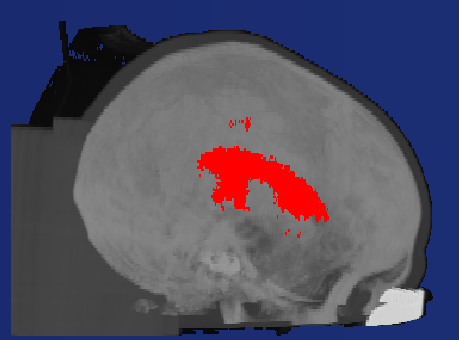
\includegraphics[width=\textwidth]{Logos/Normal1/Seite.PNG}
\captionof{figure}{Visualisierung des ersten normalen Ventrikelsystems von der Seite}
\label{fig:norm1_s}
\end{minipage}
\begin{minipage}[t]{0.49\textwidth}
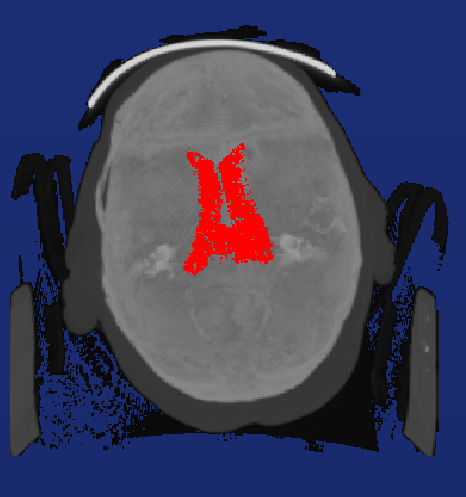
\includegraphics[width=\textwidth]{Logos/Normal1/Unten.PNG}
\captionof{figure}{Visualisierung des ersten normalen Ventrikelsystems von Unten}
\label{fig:norm1_u}
\end{minipage}

\begin{figure}[H]
\begin{minipage}[b]{.5\textwidth}
  \centering
  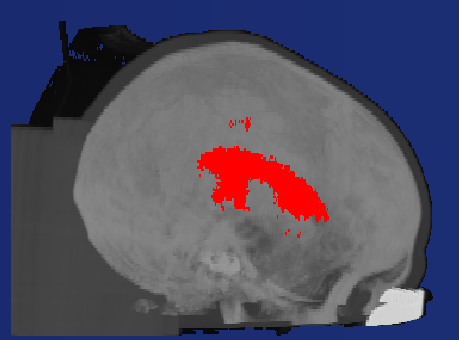
\includegraphics[width=.9\linewidth, height=.9\linewidth]{Logos/Normal1/Seite.PNG}
  \caption{A figure}
  \label{fig:test1}
\end{minipage}%
\begin{minipage}[b]{.5\textwidth}
  \centering
  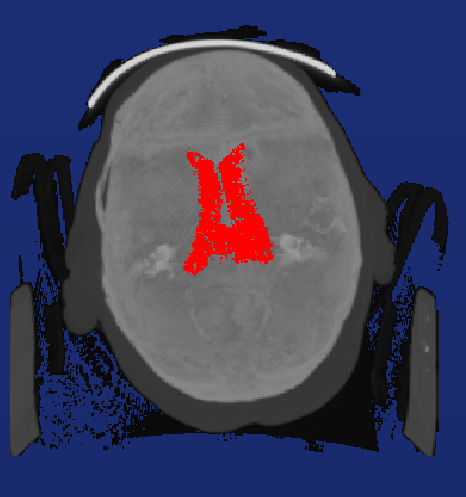
\includegraphics[width=.9\linewidth, height=.9\linewidth]{Logos/Normal1/Unten.PNG}
  \caption{Another figure}
  \label{fig:test2}
\end{minipage}
\end{figure}


In \autoref{fig:norm1_s}, der Darstellung des ersten normalen Ventrikelsystems von der Seite, sind links über dem Hinterhorn der Seitenventrikel Punkte zu erkennen, die nicht zum Ventrikelsystem gehören. Auch bei den Visualisierungen der andern Ventrikelsysteme sind an mehreren Stellen solche Ausreißer zu erkennen. Diese können bei dem aktuellen Stand der Implementierung nicht entfernt werden und senken die Qualität der Darstellung. 


\begin{minipage}[t]{0.49\textwidth}
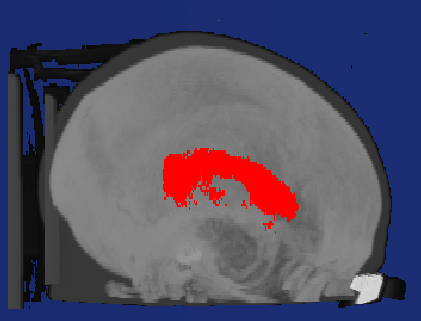
\includegraphics[width=\textwidth]{Logos/Normal2/Seite.PNG}
\captionof{figure}{Visualisierung des zweiten normalen Ventrikelsystems von der Seite}
\label{fig:norm2_s}
\end{minipage}
\begin{minipage}[t]{0.49\textwidth}
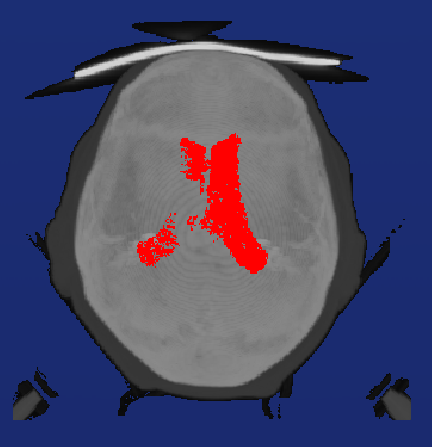
\includegraphics[width=\textwidth]{Logos/Normal2/Unten.PNG}
\captionof{figure}{Visualisierung des zweiten normalen Ventrikelsystems von Unten}
\label{fig:norm2_u}
\end{minipage}



\begin{minipage}[t]{0.49\textwidth}
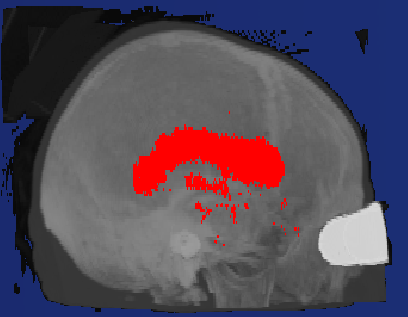
\includegraphics[width=\textwidth]{Logos/Atrophie/Seite.PNG}
\captionof{figure}{Visualisierung des Atrophie Ventrikelsystems von der Seite}
\label{fig:atro_s}
\end{minipage}
\begin{minipage}[t]{0.49\textwidth}
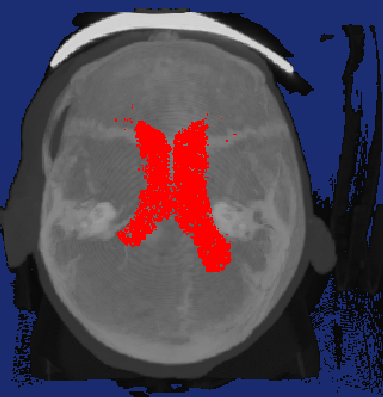
\includegraphics[width=\textwidth]{Logos/Atrophie/Unten.PNG}
\captionof{figure}{Visualisierung des Atrophie Ventrikelsystems von Unten}
\label{fig:atro_u}
\end{minipage}

\subsubsection{Datensätze}

Das Verfahren wurde an 15 verschiedenen CT-Datensätzen der Uni Ulm getestet. Darunter waren verschiedene Ventrikelsysteme.
\newline
Vier der Datensätze waren von Menschen mit einem normalen Ventrikelsystem, vier andere wiesen ein sehr schlankes System auf. Weiterhin litten zwei Patienten unter Atrophie, einem, oft durch das Alter verursachtem, Schwund an Gehirnmasse.
\newline
Zwei andere Datensätze waren von Leuten, die unter einem Mittellinienshift litten. Dies bezeichnet die Verschiebung der Mittellinie der Ventrikelsystems, was beispielsweise durch einen Schlag auf den Kopf hervorgerufen werden kann.
\newline
Des Weiteren gab es Daten, von einer Hirnblutung, und einem Hydrocephalus, einer Aufstauung von Nervenwasser im Kopf. Als letztes gab es noch Daten eines deformierten Ventrikelsystems, ausgelöst durch Wassereinlagerungen im Gehirn.


Da die Aufgabe das Ventrikelsystem anhand von CT-Daten automatisiert zu segmentieren sehr komplex ist, kam es bei Patienten mit besonderen Ventrikelsystemen zu Problemen. Da das Verfahren Strukturen anhand ihrer Grenzen erkennt, war es nicht möglich schlanke Ventrikelsysteme zu segmentieren. Da diese sehr dünn sind können sie nicht als Struktur erkannt werden.
Atrophie ist ein, oft durch das Alter verursachter, Schwund an Gehirnmasse. Bei diesem weitet sich das Ventrikelsystem und es ist im allgemeinem mehr Liquor im Gehirn zu finden. Dadurch war es bei einem der beiden Datensätze nicht möglich, das Ventrikelsystem zu segmentieren, da durch die viele Flüssigkeit im Gehirn die Grenze zwischen dem System und der umliegenden Hirnmasse nicht klar auszumachen ist.


\subsubsection{Interview mit einem Arzt}

Um die Qualität erzeugten Segmentierungen zu evaluieren, wurde ein Arzt von der Uniklinik Ulm interviewt. Diesem wurden die drei gezeigten Visualisierungen direkt in Unity vorgeführt. Während der Vorführung konnte der Mediziner selbst die Kamera durch die Darstellung lenken und das Ergebnis aus verschiedenen Blickwinkeln betrachten.
\newline
Anschließend bewertete er die Qualität der Ergebnisse, indem er drei verschiedenen Fragen zu den Darstellungen beantwortete. Er musste dabei seine Antwort immer auf einer Skala von 1 bis 5 angeben.
\newline
Die Fragen lauteten:
\begin{itemize}
	\item 1) Wie gut ist das Ventrikelsystem bei der Visualisierung zu erkennen? \newline sehr schlecht 1 - 5 sehr gut
	\item 2) Wird das Ventrikelsystem in der Visualisierung vollständig dargestellt? \newline überhaupt nicht vollständig 1 - 5 vollständig
	\item 3) Wie genau ist das Ventrikelsystem segmentiert? \newline überhaupt nicht segmentiert 1 - 5 ausschließlich das Ventrikelsystem ist segmentiert
\end{itemize}


Die Ergebnisse der Antworten des Arztes werden in \autoref{tab:ergebnis_arzt} gezeigt. Allgemein merkte der Mediziner jedoch an, dass bei jeder Visualisierung, die durch das Verfahren erzeugt wurde, nur der linke und rechte Seitenventrikel zu sehen war. Die deutlich schmaleren dritten und vierten Ventrikel und die Unterhörner der Seitenventrikel fehlten bei den Darstellungen komplett.
\newline
Er erklärte jedoch, dass diese bei einem gesunden Menschen sehr dünn und deshalb anhand von CT-Daten schwer zu segmentieren seien. Weiterhin sind, wie schon erwähnt, die Seitenventrikel entscheidend für eine erfolgreiche Punktion.
\newline
In folge dessen, wurde sich darauf verständigt, dass die Beantwortung der zweiten Frage, nach der Vollständigkeit des Ventrikelsystems, lediglich auf die Vollständigkeit der beiden Seitenventrikel bezogen ist.

\begin{table}[h]
\centering
\tiny
\resizebox{\columnwidth}{!}{
 \begin{tabular}{| c | c | c | c |}
  \hline
  Ventrikelsystem & 1. Frage & 2.Frage & 3. Frage\\ \hline
  Normal 1 & 4 & 4 & 3 \\ \hline
  Normal 2 & 4 & 2 & 3\\ \hline
  Atrophie & 4 & 3 & 2 \\ \hline
 \end{tabular}
 }
\caption{Ergebnisse des Interviews mit einem Arzt}
\label{tab:ergebnis_arzt}
\end{table}


Die Bewertung des ersten normalen Ventrikelsystems fiel positiv mit 11 von 15 möglichen Punkten aus. Das Ventrikelsystem war als solches klar und deutlich zu erkennen, jedoch fehlte ein Teil der Hinterhörner. Bis auf diese waren die Seitenventrikel jedoch vollständig zu sehen. Weiterhin war die Segmentierung nicht exakt, da es mehrere kleine Ausreißer gab.
\newline
Das zweite normale Ventrikelsystem, war ebenfalls klar zu erkennen. Jedoch wurde fast ausschließlich der linke Seitenventrikel segmentiert. Die Bewertung der Vollständigkeit fiel mit einer vier so hoch aus, da der eine Seitenventrikel sehr klar, deutlich und vollständig zu sehen war. Der Arzt sagte, dass dieser besser und glatter als die des ersten normalen Ventrikelsystems sein, da auch das Hinterhorn zu erkennen ist. 
\newline
In einem Gehirn eines unter Atrophie leidenden Menschen, ist deutlich mehr Liquor, als bei einem gesunden Menschen, zu finden. Diese Flüssigkeiten werden vom Verfahren ebenfalls erkannt, weshalb die Segmentierung etwas verschwommen erscheint und nicht die kompletten Seitenventrikel erfasst werden. Jedoch vermutete der Arzt, dass viele der Ausreißer zum dritten Ventrikel gehören könnten, da sich dieses, wie alle Ventrikel bei einer Atrophie, weitet. Trotz der Flüssigkeiten im Gehirn war das Ventrikelsystem in der Darstellung deutlich zu erkennen.
\newline
Im Allgemeinen bemängelte der Arzt, dass die Darstellungen nicht glatt genug sei und viele Ausreißer existieren. Jedoch sagte der Mediziner, dass das Ventrikelsystem bei allen Segmentierungen eindeutig zu erkennen sei.

\subsubsection{Weitere Auswertungen}

Zur weiteren Auswertung der Ergebnisse wurde das erste normale Ventrikelsystem aus \autoref{fig:norm1_s} und \autoref{fig:norm1_u} in Unity und mit der MITK-Workbench, die auch zum Umwandeln der DICOM-Dateien benutzt wurde, visualisiert.
\newline
In Unity wurde dabei die Erweiterung zum hervorheben von Wertebereichen benutzt. Diese wurde auf 1025 bis 1030 eingestellt, da das Ventrikelsystem Intensitätswerte in diesem Bereich hat. Dieses Vorgehen entspricht einer simplen eindimensionalen Transferfunktion, die abhängig von den Intensitätswerten Voxel einfärbt.
\newline
Die Ergebnisse sind in \autoref{fig:unity_s} und \autoref{fig:unity_u} zu sehen. Das Ventrikelsystem ist zwar zu sehen, es gibt jedoch sehr viele Ausreißer, die es fast unmöglich machen die Ventrikel eindeutig zu erkennen. Diese simple Vorgehensweise führt zu keinem gewünschtem Ergebnis.


\begin{minipage}[t]{0.49\textwidth}
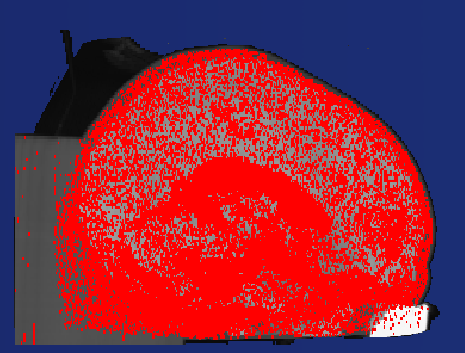
\includegraphics[width=\textwidth]{Logos/Normal1_Unity/Seite.PNG}
\captionof{figure}{Visualisierung des ersten normalen Ventrikelsystems von der Seite mithilfe von Unity}
\label{fig:unity_s}
\end{minipage}
\begin{minipage}[t]{0.49\textwidth}
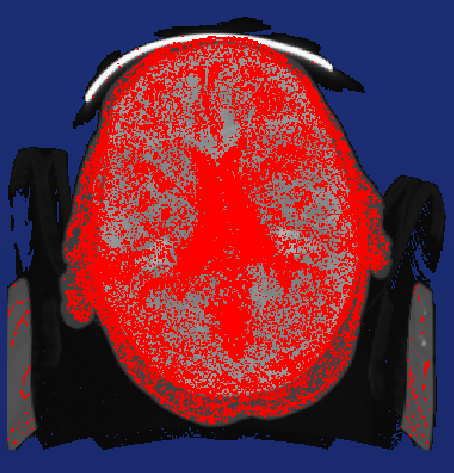
\includegraphics[width=\textwidth]{Logos/Normal1_Unity/Unten.PNG}
\captionof{figure}{Visualisierung des zweiten normalen Ventrikelsystems von Unten mithilfe von Unity}
\label{fig:unity_u}
\end{minipage}


In der MITK-Workbench gibt es verschiedene Segmentierungstools. Darunter ist ein Region Growing Tool, bei dem der Nutzer einen \textit{seed} Punkt in den Schnittbildern wählen kann. Über die verwendete Kostenfunktion werden keine Informationen genannt.
\newline
Anschließend können die Löcher der Auswahl mit einem \textit{closing} Filter geschlossen und mit einem weiteren Tool ein geglättete 3D Ansicht des Ergebnis erzeugt werden.
\newline
Screenshots der Ergebnisse sind in \autoref{fig:mitk_o} und \autoref{fig:mitk_v} zu sehen. Eine genaue Beschreibung, über das Anwenden der Tools, ist im Anhang diese Arbeit zu finden.
\newline
In dem von der Workbench erzeugte Ergebnis ist das Ventrikelsystem gut zu erkennen. Die Seitenventrikel sind vollständig und besitzen eine glatte Oberfläche. Sogar große Teile des dritten und vierten Ventrikels sind teil der Segmentierung.
\newline
Allerdings sind auch ganze Bereiche hervorgehoben, die nicht zum Ventrikelsystem gehören. Diese könnten vom Benutzer manuell in jedem Schichtbild des Datensatzes entfernt werden, was jedoch sehr zeitaufwändig wäre.


\begin{minipage}[t]{0.49\textwidth}
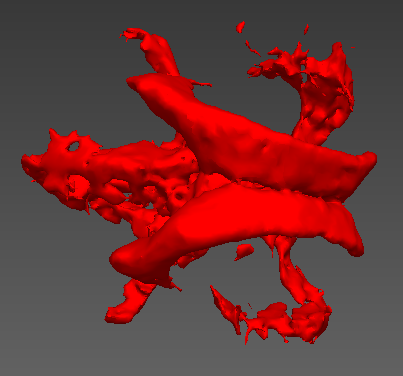
\includegraphics[width=\textwidth]{Logos/Normal1_MITK/Oben.PNG}
\captionof{figure}{Visualisierung des ersten normalen Ventrikelsystems von Oben mithilfe von MITK}
\label{fig:mitk_o}
\end{minipage}
\begin{minipage}[t]{0.49\textwidth}
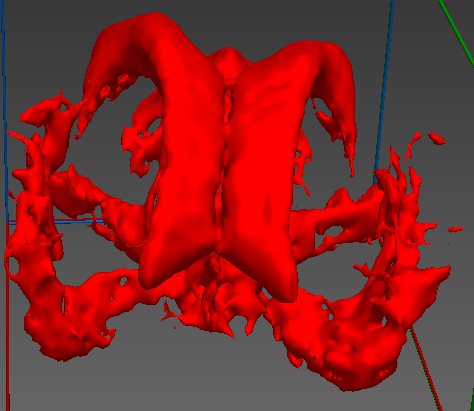
\includegraphics[width=\textwidth]{Logos/Normal1_MITK/Schraeg_Vorne.PNG}
\captionof{figure}{Visualisierung des ersten normalen Ventrikelsystems von Vorne mithilfe von MITK}
\label{fig:mitk_v}
\end{minipage}


\subsection{Nutzerstudie}


Im Rahmen der Evaluation der Benutzerfreundlichkeit des Verfahrens wurde eine kleine Nutzerstudie mit 5 Teilnehmern durchgeführt. Die Probanden waren alle Studenten aus verschiedenen Studiengängen im Alter zwischen 22 und 26 Jahren.
\newline
Als erstes wurden den Teilnehmern der Ablauf und die vom Benutzer erforderlichen Schritte, um eine Visualisierung des Ventrikelsystems zu erhalten, mittels einer Vorführung durch den Interviewer gezeigt.
\newline
Anschließend mussten die Probanden selbst das eben gelernte anwenden und das Programm selber ausführen. Dabei bekamen sie, wenn sie nicht weiterwussten, Hilfe vom Versuchsleiter.
\newline
Hinterher füllten die Teilnehmer einen NASA-TLX Bogen zu der Aufgabe aus. Dieser besteht aus zwei Parts. Als erstes muss der Befragte in den Kategorien Geistige Anforderung, Körperliche Anforderung, Zeitliche Anforderung, Leistung, Anstrengung und Frustration die auszuführende Aufgabe jeweils auf einer Skala von 5 bis 100 bewerten. Die Werte der Skalen wachsen dabei in Fünfer Schritten an. Diese Bewertung ergibt hinterher die Gewichtung der Kategorien.
\newline
Als zweites werden alle Kategorien paarweise miteinander verglichen und der Probanden muss angeben, welcher der beiden Kategorien für das Lösen der Aufgabe bedeutsamer war. Dadurch erhält jede Kategorie eine Anzahl an Klicks.
\newline
Anschließend wird die Klickzahl durch 15, die Anzahl aller Klicks geteilt. Dies ergibt die die Wichtung der Kategorie. Diese Wichtungen werden mit deren jeweiligen Gewichtungen multipliziert und die Ergebnisse zur Gesamtbeanspruchung der Aufgabe aufaddiert.
\newline
Die durchschnittlichen Ergebnisse der einzelnen Kategorien werden in \autoref{tab:ergebnis_nasa} gezeigt.


\begin{table}[H]
\centering
\resizebox{\columnwidth}{!}{
 \begin{tabular}{| c | c | c | c |}
  \hline
  Kategorie & Gewichtung & Klicks & Wichtung \\ \hline
  Geistige Anforderung & 39 & 4,8 & 0,32 \\ \hline
  Körperliche Anforderung & 23 & 1,8 & 0,12\\ \hline
  Zeitliche Anforderung & 29 & 1,2 & 0,078 \\ \hline
  Leistung & 25 & 2,4 & 0,156\\ \hline
  Anstrengung & 36 & 2,4 & 0,156\\ \hline
  Frustration & 35 & 2,4 & 0,156\\ \hline 
 \end{tabular}
 }
\caption{Durchschnittlichen Ergebnisse des NASA-TLX Bogens}
\label{tab:ergebnis_nasa}
\end{table}


Der durchschnittliche Wert für die Gesamtbeanspruchung lag bei 38,32. 


Zunächst werden die Ergebnisse des ersten Teils betrachtet. Hierbei fällt als erstes auf, dass die bei Kategorien Geistige Anforderung, Anstrengung und Frustration durchschnittlichen die höchsten Bewertungen abgegeben wurden.
\newline
Bei der Geistigen Anforderung und der Frustration gaben vor allem die Teilnehmer ohne oder mit nur wenig Programmiererfahrung höhere Werte an. Bei der Kategorie Anstrengung ist anzumerken, dass von zwei Probanden deutlich höhere Werte als vom Rest gegeben wurde.
\newline
Alle anderen Kategorien wurden in etwa ähnlich bewertet.


Als nächstes werden die Ergebnisse des zweiten Parts diskutiert. Die höchste durchschnittliche Klickzahl wurde von der Kategorie Geistige Anforderung erzielt. Unabhängig von den Programmierkenntnissen der Probanden, wurde diese Kategorie als die deutlich bedeutsamste angesehen.
\newline
Die anderen Kategorien unterscheiden sich nur geringfügig und hatten meist Klickzahlen zwischen null und drei.


Als letztes wird die Gesamtbeanspruchung betrachtet. Dieser unterscheidet sich bei den Teilnehmern, vor allem durch die unterschiedliche Bewertung der Kategorien Geistige Anforderung und Frustration, sehr stark von einander.
\newline
Die berechneten Gesamtbeanspruchungen lagen bei 14,6\; 27,3\; 40\; 40,6 und 63. Dies zeigt den großen Unterschied zwischen den Leuten, die viel Programmiererfahrungen besitzen, und denen, die wenig oder noch nie programmiert haben.


Die Benutzung einer Konsole fiel den Unerfahrenen vergleichsweise sehr schwer. Des Weiteren ist die Notwendigkeit die richtigen Suffixe und das $u$ beim \textit{ClusterVolume} Modul angeben zu müssen eine Hürde. Weiterhin wäre es einfacher wenn nur ein Programm verwendet werden müsste.

 
Trotz der Schwierigkeiten, gaben alle Probanden, auch jene ohne Programmiererfahrung, an, dass sie die Aufgabe mit einer gut erklärten, ausführlichen Dokumentation alleine, ohne weitere Hilfe zu benötigen, hinbekommen würden.

\newpage
\subsection{Berechnungszeit}

Die in diesem Unterkapitel vorgestellten Zeitmessungen wurde alle auf einem Computer mit einem 3.70GHz  Intel Core(TM) i7-8700K CPU mit 32GB RAM ausgeführt.
\newline
Um die Berechnungszeit des Systems evaluieren zu können, wurde die Kalkulation des gesamten Clusteringverfahrens sowie die Berechnung des LH-Histogramms auf drei Volumen verschiedener Größen durchgeführt. Damit der Vergleich nicht von unterschiedlichen Volumendaten verfälscht wird, wurden alle Volumen aus dem gleichen CT-Datensatz generiert.
\newline
Dabei wurde die Originalgröße, die ein Auflösung von 512x201x512 Pixeln besitzt, mithilfe des Resamplemoduls des Helpers verkleinert. Die beiden anderen Volumengrößen haben dabei die  Hälfte, mit 256x101x256 Pixeln, und Dreiviertel, mit 384x151x384 Pixeln, der Auflösungen des Originalvolumens.
\newline
Es war geplant, dass noch ein viertes Volumen zum Vergleich hinzugezogen wird. Jedoch war es aus einem unbekannten Fehler nicht möglich die beiden Berechnungen mit dem gevierteltem Volumen durchzuführen.
\newline
Des Weiteren funktionierte beim Originalvolumen lediglich die Berechnung des LH-Histogramms. Die Kalkulation des Clusteringverfahrens war nicht möglich, vermutlich aus dem Grund, dass bei dieser hohen Auflösung es zu viele Daten für die aktuelle Implementierung zu berechnen gab.
\newline
Die Berechnungszeit hängt stark von der Größe des Eingabevolumens ab. Die ist in \autoref{tab:ueberblick_zeit} sehr gut zu erkennen. Diese zeigt einen Überblick über die  Berechnungszeiten der verschiedenen Volumengrößen.


\begin{table}[h]
\centering
\resizebox{\columnwidth}{!}{
 \begin{tabular}{| c | c | c | c |}
  \hline
  Volumengröße & LH-Histogramm $[s]$ & Komplettes Verfahren $[s]$ \\ \hline
  Halbes Volumen (256x101x256)  & 30 &  50	\\ \hline
  Dreiviertel Volumen (384x151x384)  & 90 &  380	\\ \hline
  Ganzes Volumen (512x201x512) & 225 & -	\\ \hline
 \end{tabular}
 }
\caption{Überblick über die Berechnungszeiten der verschiedenen Volumengrößen}
\label{tab:ueberblick_zeit}
\end{table}


Dabei ist wichtig zu beachten, dass die Zeit zur Berechnung der LH-Histogramme die gleiche Zeit wie die Kalkulation der LH-Werte im gesamten Verfahren benötigt. Die Berechnungsdauer der Gradienten ist hierbei zirka doppelt so lange wie die der LH-Werte. Wird die Berechnungszeit des Histogramms von der Kalkulationszeit des gesamten Verfahrens abgezogen, ergibt dies die Zeit die die Beiden Clusteringschritte benötigen.
\newline
Eine interessante Beobachtung hierbei ist, dass die Berechnung der LH-Histogramme abhängig von der Anzahl der Pixel gesehen in etwa gleich schnell abläuft. Das halbe Volumen hat eine Gesamtpixelzahl von ungefähr 6,6 Millionen, das dreiviertel Volumen von zirka 22,2 Millionen und das Original von grob 52,6 Millionen Pixeln.
\newline
Wird die Anzahl an Pixeln die pro Sekunde bei der LH-Wert Berechnung bearbeitet werden für diese drei Volumen berechnet, so ist zu beobachten, dass keine großen Unterschied zwischen den Zeiten existiert.
\newline
Das Halbe bearbeitet etwa 220 Tausend, das Dreiviertel ungefähr 247 Tausend und das Ganze 234 Tausend Pixel pro Sekunde. Der kleine Unterschied in der Rate lässt sich einerseits durch von der Volumengröße unabhängige Berechnungen, und andererseits durch Messfehler erklären. Folglich kann die Aussage getroffen werden, dass die Berechnungszeit der LH-Werte bei dieser Implementierung in etwa linear mit der Anzahl an Eingabepixeln wächst.
\newline
Auf der anderen Seite ist jedoch auch zu erkennen, dass die beiden Clusteringschritte mit zunehmender Eingabegröße deutlich langsamer werden. Das Clustering des halben Volumens dauerte 20 Sekunden und hat damit eine Verarbeitungsrate von zirka 330 Tausend Pixeln pro Sekunde. Hingegen dauert es beim dreiviertel Volumen 290 Sekunden und erreicht damit gerade einmal einen Rate von 76 Tausend Pixeln pro Sekunde. Es benötigt also 14,5 mal so viel Zeit für die 3,3 fache Anzahl an Pixeln.















































%% ==============================
\chapter{\iflanguage{ngerman}{Fazit}{Discussion}}
\label{sec:discussion}
%% ==============================


Nachdem die Ergebnisse im vorherigen Kapitel gezeigt und evaluiert wurden, wird in diesem ein Fazit gezogen.
\newline
Das Ziel der Bachelorarbeit, war die Implementierung eines Verfahrens zur erfolgreiche Segmentierung des Ventrikelsystem basierend auf Volumendaten. Dieses Ziel wurde erfüllt.
\newline
Das Ventrikelsystem ist in den Visualisierungen deutlich sehen und als solches auch klar zu identifizieren. Die beiden für die Operation essentiell wichtigen Seitenventrikel werden hervorgehoben.
Es fehlten zwar bei allen Visualisierungen der dritte und vierte Ventrikel, jedoch sind diese für die Ventrikelpunktion nicht von Nöten. Das Hervorheben soll den Arzt im Operationssaal assistieren. Dazu sollte ihm nach Möglichkeit nur für den Eingriff relevante Informationen angezeigt werden. Er könnte die  Übersicht verlieren, wenn ihm der, für die Operation irrelevanten, dritte und vierte Ventrikel angezeigt werden würden. Dies würde einen erfolgreichen Eingriff gefährden.
\newline
Das Verfahren konnte bei mehreren Datensätzen zu keiner erfolgreichen Segmentierung gelangen. Dies lag jedoch an der Besonderheit der verschiedenen Datensätze, bei denen es oftmals schwer bis nicht möglich war nur anhand der CT-Daten zu einer Segmentierung zu gelangen.
\newline
Die Schritte, die vom Benutzer ausgeführt werden müssen, um zu einem Ergebnis zu gelangen, sind wenig intuitiv. Er benötigt Wissen darüber welche Befehle wann im Helper ausgeführt werden müssen deren Syntax und die passenden Dateiformate. Außerdem muss der Anwender die passenden IDs manuell finden, was zeitaufwändig sein kann.
\newline
Trotzdem zeigte die Nutzerstudie, dass selbst Menschen ohne Programmiererfahrung die Aufgabe bewältigen können. Des Weiteren ist die Ausführung des Verfahrens mit einer guten Dokumentation auch ohne weitere Hilfe durchführbar. Nach einer kleinen Eingewöhnungsphase sollte das Durchführen für den Anwender kein Problem darstellen.
Trotzdem könnte versucht werden, die Anwendung einfacher und intuitiver zu gestalten. Dies ist noch nicht geschehen, da beim Arbeiten an der Implementierung die Funktionalität oberste Priorität hatte.
\newline
Schließlich wird noch die Verarbeitungsgeschwindigkeit des Verfahren betrachtet. Diese ist für die kleineren Auflösungen relativ schnell. Die benötigte Zeit zur Berechnung der Cluster wächst jedoch nicht linear mit der Größe der Eingabe. Hierbei ist jedoch unklar, ob dies an der Implementierung oder an dem Verfahren an sich liegt, da über die Laufzeit des \textit{Meanshiftclustering} keine Informationen vorliegen.


Zusammenfassend lässt sich sagen, dass die Bachelorarbeit zu einem positiven Ergebnis gelangt ist. Es war möglich die, im Kontext des HoloMed Projektes, wichtigen Bereiche des Ventrikelsystems zu segmentieren und hervorzuheben.
\newline
In einer anschließenden Arbeit kann das Verfahren noch weiter verbessert werden. Ein Ausblick wie die verschiedenen genannten Probleme behoben und verbessert werden können wird im nächsten Kapitel gegeben.


























%% ==============================
\chapter{\iflanguage{ngerman}{Zusammensaffung und Ausblick}{Conclusion}}
\label{sec:conclusion}
%% ==============================

\dots




%% --------------------
%% |   Bibliography   |
%% --------------------
\Bibliography{Bibliography/thesis}

%% ----------------
%% |   Appendix   |
%% ----------------
% \cleardoublepage
%% appendix.tex
%%

%% ==============================
\Appendix
\label{ch:Appendix}
%% ==============================



\section{First Appendix Section}
		\label{Anhang-Implementierung}



\begin{figure} [ht]
  \centering
   ein Bild
  \caption{A figure}
  \label{fig:BPMNBeispiela}
\end{figure}


\dots





\end{document}
